\documentclass[11pt, chapterprefix, headsepline]{scrartcl}

% for arXiv
\pdfoutput=1

\usepackage{graphicx,amssymb,amsmath,multirow,amsfonts,amsthm,latexsym,graphics}
% Include figure files

\usepackage{tabularx}
\usepackage{tabulary}

\usepackage{amsmath}
\usepackage{natbib}
%\usepackage{auto-pst-pdf}
%\usepackage{psfrag, color, epsfig, rotating, pstricks, pst-node}
\usepackage{color}
\usepackage{dsfont}
\usepackage{txfonts}
\usepackage{ulem}
\usepackage{longtable}
%\usepackage{a4wide}
\usepackage{ifthen}
\usepackage{dsfont}
\usepackage{mathtools}

%\usepackage{typearea}

% SCRBook
%change to
%in texititel.sty for newest latex versions
% arxiv: renewcommand
% Martin: newcommand
% Jean: comment
\usepackage{texititel}
\newcommand{\mysubtitle}[1]{\renewcommand{\TexiSubTitle}{#1}}

% Hyperref
\usepackage[pagebackref, breaklinks]{hyperref}
\usepackage[hyperpageref]{backref} 

\definecolor{dark-red}{rgb}{0.4,0.15,0.15}
\definecolor{dark-blue}{rgb}{0.15,0.15,0.4}
\definecolor{medium-blue}{rgb}{0,0,0.5}

% The following makes AdobeReader crash, so we comment it out (v >= 1.3)
%\hypersetup{%
  %pdftitle    = {CosmoPMC},
  %pdfsubject  = {Cookbook},
  %pdfauthor   = {Martin Kilbinger},
  %pdfkeywords = {Monte Carlo, sampling, Baysian, statistics},
  %pdfcreator  = {LaTeX v3.141592},
  %pdfproducer = {pdflatex},
  %%colorlinks,
  %%linkcolor={dark-red},
  %%citecolor={dark-blue},
  %%urlcolor={medium-blue}
  %pdfborder   = {0 0 0.5 [0.3 0.3]},
 %}

\input preliminaries

% Counters for the hyperlinks
\newcounter{addcommenttopsplc}\setcounter{addcommenttopsplc}{1}
\newcounter{adddedplc}\setcounter{adddedplc}{1}
\newcounter{adddeducedcosebisc}\setcounter{adddeducedcosebisc}{1}
\newcounter{adddeducedhalomodelc}\setcounter{adddeducedhalomodelc}{1}
\newcounter{addpartomvdensplc}\setcounter{addpartomvdensplc}{1}
\newcounter{addparfrompriorplc}\setcounter{addparfrompriorplc}{1}
\newcounter{addpmcproposalc}\setcounter{addpmcproposalc}{1}
\newcounter{bayesfactorplc}\setcounter{bayesfactorplc}{1}
\newcounter{clonesidedc}\setcounter{clonesidedc}{1}
\newcounter{corrcoeffshc}\setcounter{corrcoeffshc}{1}
\newcounter{configpmctomaxandfishplc}\setcounter{configpmctomaxandfishplc}{1}
\newcounter{cosmopmcc}\setcounter{cosmopmcc}{1}
\newcounter{cosmopmcplc}\setcounter{cosmopmcplc}{1}
\newcounter{diagmvdensplc}\setcounter{diagmvdensplc}{1}
\newcounter{essentialcosmopmcrunplc}\setcounter{essentialcosmopmcrunplc}{1}
\newcounter{evidencelistplc}\setcounter{evidencelistplc}{1}
\newcounter{evidenceplc}\setcounter{evidenceplc}{1}
\newcounter{gofishingc}\setcounter{gofishingc}{1}
\newcounter{haloplotc}\setcounter{haloplotc}{1}
\newcounter{fishertomeanvarplc}\setcounter{fishertomeanvarplc}{1}
\newcounter{histogramssamplec}\setcounter{histogramssamplec}{1}
\newcounter{importancesamplec}\setcounter{importancesamplec}{1}
\newcounter{maxpostc}\setcounter{maxpostc}{1}
\newcounter{meanvarsamplec}\setcounter{meanvarsamplec}{1}
\newcounter{meantepsplc}\setcounter{meantepsplc}{1}
\newcounter{meanvartotabplc}\setcounter{meanvartotabplc}{1}
\newcounter{neffproposalplc}\setcounter{neffproposalplc}{1}
\newcounter{newdirpmcshc}\setcounter{newdirpmcshc}{1}
\newcounter{plotconfidenceRc}\setcounter{plotconfidenceRc}{1}
\newcounter{plotcontourzdplc}\setcounter{plotcontourzdplc}{1}
\newcounter{pmcsimcatplc}\setcounter{pmcsimcatplc}{1}
\newcounter{proposalmeanplc}\setcounter{proposalmeanplc}{1}
\newcounter{proposalvarplc}\setcounter{proposalvarplc}{1}
\newcounter{remapshc}\setcounter{remapshc}{1}
\newcounter{sampletofixparplc}\setcounter{sampletofixparplc}{1}
\newcounter{samplefrompmcsimuRc}\setcounter{samplefrompmcsimuRc}{1}
\newcounter{tabtotexplc}\setcounter{tabtotexplc}{1}

% Sets a reference hyperlink
\newcommand*{\ttrefc}[3]{%
 % links as 'n#2': for some reason, links which start with some 
  %  specific letters (e.g. 'c', 'p') don't work
\hyperlink{n#2}{\progr{#2}}%
  \label{#3-#1}%
  \refstepcounter{#1c}%
}

% Writes text, sets a target (for corresponding hyperlink) and sets #3
% number of back references
\newcommand*{\ttback}[3]{%
  %
  \addtocounter{#1c}{-1}
  \hypertarget{n#2}{\progr{#2}}\hspace*{2ex}%
  %
  \hyperref[1-#1]{\pageref*{1-#1}}%
  %
  \ifthenelse{\equal{#3}{2}}{%
    , \hyperref[2-#1]{\pageref*{2-#1}} }{}%
  %
  \ifthenelse{\equal{#3}{3}}{%
    , \hyperref[2-#1]{\pageref*{2-#1}}, \hyperref[3-#1]{\pageref*{3-#1}} }{}%
  %
  \ifthenelse{\equal{#3}{4}}{%
    , \hyperref[2-#1]{\pageref*{2-#1}}, \hyperref[3-#1]{\pageref*{3-#1}}, \hyperref[4-#1]{\pageref*{4-#1}} }{}%
  %
}

\def\sun{\hbox{$\odot$}}
\newcommand{\ud}{\mathrm{d}}
\newcommand{\SUBSECTION}[1]{\subsection{#1}}
\newcommand{\REF}[3]{#1\ref{#2}#3}
\newcommand{\onlyif}[2]{\footnote{only if \texttt{#1 =\; #2}}}
\newcommand{\notif}[2]{\footnote{not if \texttt{#1 =\; #2}}}
\newcommand{\mythemp}{$^{\renewcommand{\thempfootnote}{\alph{mpfootnote}}\thempfootnote}$}
\bibpunct{(}{)}{;}{a}{}{,}


\setlength{\parindent}{0in}
\addtolength{\parskip}{0.3\baselineskip}




%%%%%%%%%%%%%%%%%%%%%%%%%%%%%%%%%%%%%%%%%%%%%%%%%%%%%%%%%%%%
%%%%%%%%%%%%%%%%%%%%%%%%%%%%%%%%%%%%%%%%%%%%%%%%%%%%%%%%%%%%
\begin{document}
%%%%%%%%%%%%%%%%%%%%%%%%%%%%%%%%%%%%%%%%%%%%%%%%%%%%%%%%%%%%
%%%%%%%%%%%%%%%%%%%%%%%%%%%%%%%%%%%%%%%%%%%%%%%%%%%%%%%%%%%%

\input abbr-journals


%%%%%%%%%%%%%%%%%%%%%%%%%%%%%%%%%%%%%%%%%%%%%%%%%%%%%%%%%%%%
%\begin{titlepage}
%\titlehead{Kopf}
%\extratitle{\CosmoPMC}
\setcounter{page}{0}

%\title{\CosmoPMC\ v\CosmoPMCVersion}
%\subtitle{Cosmology Population Monte Carlo \hfill User's manual}
\title{Cosmology Population Monte Carlo}
\mysubtitle{\CosmoPMC\ v\CosmoPMCVersion\ \hfill User's manual}
%\TexiSubTitle{\CosmoPMC\ v\CosmoPMCVersion\ \hfill User's manual}
%\publishers{\CosmoPMC\ v\CosmoPMCVersion\ \hfill User's manual}

\subject{The cookbook}
\author{%
%\centerline{\includegraphics[width=5cm]{contour2d_0_1.pdf}}%
%\vspace*{1cm}%
  \parbox{\textwidth}{
    Martin Kilbinger\\
    Karim Benabed\\
    Olivier Capp\'e\\
    Jean Coupon\\
    Jean-Fran\c{c}ois Cardoso\\
    Gersende~Fort\\
    Henry J.~McCracken\\
    Simon Prunet\\
    Christian P.~Robert\\
    Darren Wraith
}
}
\date{\today}
%\end{titlepage}
\maketitle
\newpage
%%%%%%%%%%%%%%%%%%%%%%%%%%%%%%%%%%%%%%%%%%%%%%%%%%%%%%%%%%%%

\pagenumbering{roman}

\pdfbookmark[0]{\contentsname}{toc}
\setcounter{tocdepth}{2}
\setcounter{page}{0}
\tableofcontents
\setcounter{page}{0}
\newpage
\setcounter{page}{1}


\pagestyle{headings}
%\thispagestyle{plain}


%%%%%%%%%%%%%%%%%%%%%%%%%%%%%%%%%%%%%%%%%%%%%%%%%%%%%%%%%%%%
\section{What is \CosmoPMC?}
\pagenumbering{arabic}
%%%%%%%%%%%%%%%%%%%%%%%%%%%%%%%%%%%%%%%%%%%%%%%%%%%%%%%%%%%%

\hyperlink{spec}{name}

\CosmoPMC\ (Cosmology Population Monte Carlo) is a Bayesian sampling
method to explore the likelihood of various cosmological probes. The
sampling engine is implemented with the package \pmclib. It is called
Population Monte Carlo (PMC), which is a novel technique to sample from
the posterior \citep{cappe:douc:guillin:marin:robert:2007}. PMC is an
adaptive importance sampling method which iteratively improves the
proposal to approximate the posterior. This code has
been introduced, tested and applied to various cosmology data sets in
\citet{WK09}. Results on the Bayesian evidence using PMC are discussed
in \cite{KWR10}.

%%%%%%%%%%%%%%%%%%%%%%%%%%%%%%%%%%%%%%%%%%%%%%%%%%%%%%%%%%%%
\subsection{Importance sampling}
%%%%%%%%%%%%%%%%%%%%%%%%%%%%%%%%%%%%%%%%%%%%%%%%%%%%%%%%%%%%


One of the main goals in Bayesian inference is to obtain integrals of
the form
%
\begin{equation}
  \pi(f) = \int f(x) \pi(x) \dd x
  \label{pi-f}
\end{equation}
%
over the posterior distribution $\pi$ which depends on the
$p$-dimensional parameter
$x$, where $f$ is an arbitrary function with finite expectation under
$\pi$. Of interest are for example the parameter mean ($f = {\rm
  id}$) or confidence regions $S$ with $f=\indicator_{S}$ being the indicator
function of $S$. The Bayesian evidence $E$, used in model comparison
techniques, is obtained by setting $f=1$, but instead of $\pi$ using the unnormalised
posterior $\pi^\prime = L \cdot P$ in (\ref{pi-f}), with $L$ being
the likelihood and $P$ the prior.

The evaluation of (\ref{pi-f}) is challenging because
the posterior is in general not available analytically, and the
parameter space can be high-dimensional. Monte-Carlo methods to
approximate the above integrals consist in providing a sample
$\{x_n\}_{n=1 \ldots N}$
under $\pi$, and approximating (\ref{pi-f}) by the estimator
%
\begin{equation}
  \hat \pi(f) = \frac 1 N \sum_{n=1}^N f(x_n).
  \label{hat-pi-f}
\end{equation}

Markov Chain Monte Carlo (MCMC) produces a Markov chain of points for
which $\pi$ is the limiting distribution. The popular and widely-used
package \progr{cosmomc}
\citep[\url{http://cosmologist.info/cosmomc};][]{cosmomc} implements MCMC
exploration of the cosmological parameter space.

Importance sampling on the other
hand uses the identity
%
\begin{equation}
  \pi(f) = \int f(x) \pi(x) \dd x = \int f(x) \frac{\pi(x)}{q(x)} q(x) \,
  \dd x
\end{equation}
%
where $q$ is any probability density function with support including
the support of $\pi$.
%, ${\rm sup}\, q \supseteq {\rm sup}\, \pi$.
A sample $\{x_n\}$ under $q$ is then
used to obtain the estimator
%
\begin{equation}
  \hat \pi (f) = \frac 1 N \sum_{n=1}^N f(x_n) \, w_n; \;\;\;\; w_n =
  \frac{\pi(x_n)}{q(x_n)}.
  \label{eq:importance_weight}
\end{equation}
%
The function $q$ is called the \textit{proposal} or \textit{importance
  function}, the quantities $w_n$ are the \textit{importance weights}.
Population Monte Carlo (PMC)  produces a sequence $q^t$ of importance
functions ($t=1 \ldots T$) to approximate the posterior $\pi$. Details
of this algorithm are discussed in \citet{WK09}.

The package \CosmoPMC\ provides a C-code for sampling and exploring the
cosmological parameter space using Population Monte Carlo. The code
uses MPI to parallelize the
calculation of the likelihood function. There is very little overhead
and on a massive cluster the reduction in wall-clock time can be
enormous. Included in the package are post-processing, plotting and
various other analysis scripts and programs. It also provides a
Markov Chain Monte-Carlo sampler.


%%%%%%%%%%%%%%%%%%%%%%%%%%%%%%%%%%%%%%%%%%%%%%%%%%%%%%%%%%%%
\subsection{This manual}
%%%%%%%%%%%%%%%%%%%%%%%%%%%%%%%%%%%%%%%%%%%%%%%%%%%%%%%%%%%%

This manual describes the code \CosmoPMC, and can be obtained from
\url{www.cosmopmc.info}. \CosmoPMC\ is the cosmology interface to the
Population Monte Carlo (PMC) engine \pmclib. Documentation on the PMC
library can be found at the same url.
%\url{http://www2.iap.fr/users/kilbinge/CosmoPMC/pmclib}.
The cosmology module of \CosmoPMC\ can be used as stand-alone program,
it has the name \nicaea\
(\url{http://www2.iap.fr/users/kilbinge/nicaea}).

Warning: Use undocumented features of the code at your own risk!


%%%%%%%%%%%%%%%%%%%%%%%%%%%%%%%%%%%%%%%%%%%%%%%%%%%%%%%%%%%%
\section{Installing  \CosmoPMC}
%%%%%%%%%%%%%%%%%%%%%%%%%%%%%%%%%%%%%%%%%%%%%%%%%%%%%%%%%%%%

%%%%%%%%%%%%%%%%%%%%%%%%%%%%%%%%%%%%%%%%%%%%%%%%%%%%%%%%%%%%
\subsection{Software requirements}
%%%%%%%%%%%%%%%%%%%%%%%%%%%%%%%%%%%%%%%%%%%%%%%%%%%%%%%%%%%%

\CosmoPMC\ has been developed on GNU/Linux and Darwin/FreeBSD systems
and should run on those architectures. Required are:

\begin{itemize}

  \item C-compiler (e.g.~\progr{gcc}, \progr{icc})

  \item \pmclib\ (Sect.~\ref{sec:install_pmclib})

  \item GSL (\url{http://www.gnu.org/software/gsl}), version 1.15 or higher

  \item FFTW ({\url{http://www.fftw.org}})

  \item \textsc{Message Parsing Interface
      (MPI)} ({\url{http://www-unix.mcs.anl.gov/mpi}}) for parallel
    calculations

\end{itemize}

\bigskip

Optional:

\begin{itemize}

 \item \progr{csh}, for post-processing, auxiliary scripts;
    recommended

  \item \progr{perl} (\url{http://www.perl.org}), for post-processing, auxiliary scripts;
    recommended

  \item \progr{yorick} ({\url{http://yorick.sourceforge.net}}),
    post-processing, mainly plotting

  \item \progr{python} (\url{http://www.python.org}), for running the configuration script

  \item \progr{R} ({\url{http://www.r-project.org}}), post-processing

\end{itemize}

    To produce 1D and 2D marginal posterior plots with scripts that
    come with \CosmoPMC, either \progr{yorick} or \progr{R} are required.

\bigskip

Necessary for CMB anisotropies support:

\begin{itemize}

  \item Fortran compiler (e.g.~\progr{ifort})

  \item \textsc{Intel Math Kernel}
    libraries ({\url{http://software.intel.com/en-us/intel-mkl}})

  \item CAMB ({\url{http://camb.info,http://cosmologist.info/cosmomc}})

  \item WMAP data and likelihood code ({\url{http://lambda.gsfc.nasa.gov}})

\end{itemize}


%%%%%%%%%%%%%%%%%%%%%%%
\input download_install
%%%%%%%%%%%%%%%%%%%%%%%


%%%%%%%%%%%%%%%%%%%%%%%%%%%%%%%%%%%%%%%%%%%%%%%%%%%%%%%%%%%%
\section{Running \CosmoPMC}
%%%%%%%%%%%%%%%%%%%%%%%%%%%%%%%%%%%%%%%%%%%%%%%%%%%%%%%%%%%%


%%%%%%%%%%%%%%%%
\input quick_ref
%%%%%%%%%%%%%%%%


%%%%%%%%%%%%%%%%%%%%%%%%%%%%%%%%%%%%%%%%%%%%%%%%%%%%%%%%%%%%
\subsection{\CosmoPMC\ in detail}
%%%%%%%%%%%%%%%%%%%%%%%%%%%%%%%%%%%%%%%%%%%%%%%%%%%%%%%%%%%%

This section describes in more detail how PMC is run, and which
decisions the user has to make before starting and after stopping a
PMC run.


%%%%%%%%%%%%%%%%%%%%%%%%%%%%%%%%%%%%%%%%%%%%%%%%%%%%%%%%%%%%
\paragraph{Initial proposal}
\label{sec:ini_prop}
%%%%%%%%%%%%%%%%%%%%%%%%%%%%%%%%%%%%%%%%%%%%%%%%%%%%%%%%%%%%

The choice of the initial proposal, used during the first PMC
iteration, is of great importance for a successful PMC run. The
following options are implemented, determined by the key
`\texttt{sinitial}' in the configuration file (see Sect.~\ref{sec:config_file}):

\begin{enumerate}

\item \textbf{\texttt{sinitial = fisher\_rshift}} The Fisher matrix is used as the
  covariance of a multi-variate Gaussian/Student-$t$ distribution
  $g$. A mixture-model is constructed by creating $D$ copies of
  $g$. Each copy is displaced from the ML point by a random uniform
  shift, and its variance is stretched by random uniform factor.

\item \textbf{\texttt{sinitial = fisher\_eigen}} A mixture-model is constructed in a similar way as the first
  case, with the difference that the shift from the ML point is now
  performed along the major axes of the Fisher ellipsoid. Note that if the
  Fisher matrix is diagonal, the shift of each component only concerns
  one parameter.

\item \textbf{\texttt{sinitial = file}} The initial proposal is read from a file (of
  \texttt{mix\_mvdens} format), e.g. from a previous PMC run.

\item \textbf{\texttt{sinitial = random\_pos}} Mixture-model components with random variance (up to half the
  box size) and random positions. This case should only be used if the
  posterior is suspected to be multi-modal, or the calculation of the
  Fisher matrix fails.

\end{enumerate}

In many cases, a mixture of multi-variate Gaussians as the proposal is
the best choice. For that, set the degrees-of-freedom ($\nu$)
parameter \texttt{df} to -1. For a posterior with heavy tails, a
Student-$t$ distribution might be more suited. The degrees of freedom
$\nu$ can be chosen freely; $\nu = 3$ is a common choice.
For $\nu \rightarrow \infty$, a Gaussian
distribution is reached asymptotically.

If the Fisher matrix has to be calculated for the initial proposal,
the script \ttrefc{cosmopmcpl}{cosmo\_pmc.pl}{\thecosmopmcplc} calls
\ttrefc{maxpost}{max\_post}{\themaxpostc} and
\ttrefc{gofishing}{go\_fishing}{\thegofishingc} to estimate the
maximum-likelihood point and the Hessian at that point,
respectively. The script
\ttrefc{configpmctomaxandfishpl}{config\_pmc\_to\_max\_and\_fish.pl}{\theconfigpmctomaxandfishplc}
can be used to create the corresponding configuration files from the
PMC config file for manual calls of \progr{max\_post} and \progr{go\_fishing}.


%%%%%%%%%%%%%%%%%%%%%%%%%%%%%%%%%%%%%%%%%%%%%%%%%%%%%%%%%%%%
\paragraph{Updating the proposal}
%%%%%%%%%%%%%%%%%%%%%%%%%%%%%%%%%%%%%%%%%%%%%%%%%%%%%%%%%%%%

The PMC algorithm automatically updates the proposal after each
iteration, no user interference is necessary.

The method to update the proposal is a variant of the
Expectation-Maximization algorithm
\citep[EM,][]{dempster:laird:rubin:1977}. It leads to an increase of
the perplexity and an increase of ESS. Detailed descriptions of this
algorithm in the case of multi-variate Gaussian and Student-$t$
distributions can be found in
\cite{cappe:douc:guillin:marin:robert:2007} and \cite{WK09}.

%%%%%%%%%%%%%%%%%%%%%%%%%%%%%%%%%%%%%%%%%%%%%%%%%%%%%%%%%%%%
\paragraph{Dead components}
%%%%%%%%%%%%%%%%%%%%%%%%%%%%%%%%%%%%%%%%%%%%%%%%%%%%%%%%%%%%

A component can `die' during the updating if the number of points
sampled from that component is less than \texttt{MINCOUNT = 20}, or
its weight is smaller than the inverse total number of sample points
$1/N$. There are two possibilities to proceed. First, the component is
`buried', its weight set to zero so that no points are sampled from it
in subsequent iterations. Alternatively, the component can be
revived. In this case, it is placed near the component $\phi_{d_0}$
which has maximum weight, and it is given the same covariance as
$\phi_{d_0}$.

The first case is the standard method used in \cite{WK09}. The second
method tries to cure cases where the majority of components die. This
can happen if they start too far off from the high-density posterior
region. Often, only one component remains to the end, not capable of
sampling the posterior reliably.

Both options can be chosen using the config file
(Sect.~\ref{sec:config_file}) key
\texttt{sdead\_comp = \{bury|revive\}}.

%%%%%%%%%%%%%%%%%%%%%%%%%%%%%%%%%%%%%%%%%%%%%%%%%%%%%%%%%%%%
\paragraph{Errors}
\label{sec:errors}
%%%%%%%%%%%%%%%%%%%%%%%%%%%%%%%%%%%%%%%%%%%%%%%%%%%%%%%%%%%%

If an error occurs during the calculation of the likelihood, the error is
intercepted and the likelihood is set to zero. Thus, the parameter
vector for which the error occurs is attributed a zero importance
weight and does not contribute to the final sample. An error message
is printed to \file{stderr} (unless \CosmoPMC\ is run with the
option \progr{-q}) and PMC continues with the next point.

An error can be due to cosmological reasons, e.g.~a redshift is probed
which is larger than the maximum redshift in a loitering
Universe. Further, a parameter could be outside the range of a fitting
formulae, e.g.~a very small scalar spectral index in the dark matter
transfer function.

Usually, the errors printed to \file{stderr} during PMC sampling can be ignored.

%%%%%%%%%%%%%%%%%%%%%%%%%%%%%%%%%%%%%%%%%%%%%%%%%%%%%%%%%%%%
\paragraph{Random numbers}
\label{sec:random}
%%%%%%%%%%%%%%%%%%%%%%%%%%%%%%%%%%%%%%%%%%%%%%%%%%%%%%%%%%%%

The GSL random number generator is used to generate random variables.
It is initialised with a seed reading the current time, to produce
different (pseudo-) random numbers at each call. The seed is written
to the log file. Using the option '\progr{-s SEED}', a user-specified
seed can be defined. This is helpful if a run is to be repeated with
identical results.


%%%%%%%%%%%%%%%%%%%%%%%%%%%%%%%%%%%%%%%%%%%%%%%%%%%%%%%%%%%%
\subsection{Output files}
%%%%%%%%%%%%%%%%%%%%%%%%%%%%%%%%%%%%%%%%%%%%%%%%%%%%%%%%%%%%

Each iteration $i$ produces a number of output files which are stored
in subdirectories \direc{iter\_i} of the \CosmoPMC\ starting
directory. Files which are not specific to a single iteration are
placed in the starting directory.

%%%%%%%%%%%%%%%%%%%%%%%%%%%%%%%%%%%%%%%%%%%%%%%%%%%%%%%%%%%%
\subsubsection{Diagnostics}
\label{sec:diagnostics}
%%%%%%%%%%%%%%%%%%%%%%%%%%%%%%%%%%%%%%%%%%%%%%%%%%%%%%%%%%%%

Unlike in MCMC, with adaptive importance sampling one does not have to
worry about convergence. In principle, the updating process can be
stopped at any time. There are however diagnostics to indicate the quality and
effectiveness of the sampling.


%%%%%%%%%%%%%%%%%%%%%%%%%%%%%%%%%%%%%%%%%%%%%%%%%%%%%%%%%%%%
\paragraph{Perplexity and effective sample size} \quad \file{perplexity}
%%%%%%%%%%%%%%%%%%%%%%%%%%%%%%%%%%%%%%%%%%%%%%%%%%%%%%%%%%%%

The perplexity $p$ is defined in eq.~(18) of \cite{WK09}.
The range of $p$ is $[0;1]$, and will approach unity if
the proposal and posterior distribution are close together, as
measured by the Kullback-Leibler divergence. The initial perplexity is
typically very low ($<0.1$) and should increase from iteration to
iteration. Final values of 0.99 and larger are not uncommon, but also
for $p$ of about 0.6-0.8 very accurate results can be obtained. If $p$
is smaller than say 0.1, the PMC sample is most likely not
representative of the posterior. Intermediate values for $p$ are not
straight-forward to interpret.

Closely related to the perplexity is the effective sample size
$\operatorname{ESS}$, which lies in the range $[1;N]$. It is interpreted
as the number of sample point with zero weight
\citep{liu:chen:1995}. A large perplexity is usually accompanied by a
high ESS. For a successful PMC run, ESS is much higher than
the acceptance rate of a Monte Carlo Markov chain, which is typically between
0.15 and 0.25.

The file \file{perplexity} contains the iteration $i$, perplexity
$p$, ESS for that iteration, and the total ESS. This file is updated
after each iteration and can therefore be used to monitor a PMC run.

If there are points with very large weights, they can dominate the
other points whose normalised weights will be small. Even a few sample
points might dominate the sum over weights and result in a low
perplexity. The perplexity is the most sensitive quantity to those
high-weight points, much more than e.g.~the mean, the confidence
intervals or the evidence.


%%%%%%%%%%%%%%%%%%%%%%%%%%%%%%%%%%%%%%%%%%%%%%%%%%%%%%%%%%%%
\paragraph{Effective number of proposal components} \quad \file{enc}
\label{sec:prop_comp}
%%%%%%%%%%%%%%%%%%%%%%%%%%%%%%%%%%%%%%%%%%%%%%%%%%%%%%%%%%%%

The proposal $q^t$ provides useful information about the performance
of a PMC run. For example, the effective number of components, defined
in complete analogy to ESS,
%
\begin{equation}
  \operatorname{ENC} = \left( \sum_{d=1}^{D}
    \left\{\alpha_d^t\right\}^2 \right)^{-1},
  \label{enc}
\end{equation}
%
is an indication of components with non-zero weight. If ENC is close
to unity, the number of remaining components to sample the posterior
is likely to be too small to provide a representative sample.  For a
badly chosen initial proposal, this usually happens already at the
first few iterations. By monitoring the file \file{enc} which is
updated each iteration, an unsuccessful PMC run can be aborted.

The effective number of components can also be determined from any
proposal file (\texttt{mix\_mvdens} format) with the script
\ttrefc{neffproposalpl}{neff\_proposal.pl}{\theneffproposalplc}.

An additional diagnostic is the evolution of the proposal components
with iteration. This illustrates whether the components spread out
nicely across the high-posterior region and reach a more or less
stationary behaviour, or whether they stay too concentrated at one
point. The scripts
%\ttrefc{proposalmeanpl}{proposal\_mean.pl}{\theproposalmeanplc}
\ttrefc{proposalmeanpl}{proposal\_mean.pl}{\theproposalmeanplc}
(\ttrefc{proposalvarpl}{proposal\_var.pl}{\theproposalvarplc}) read in
the proposal information $q^t$ and plot the means (variances) as
function of iteration $t$.


%%%%%%%%%%%%%%%%%%%%%%%%%%%%%%%%%%%%%%%%%%%%%%%%%%%%%%%%%%%%
\subsubsection{Results}
%%%%%%%%%%%%%%%%%%%%%%%%%%%%%%%%%%%%%%%%%%%%%%%%%%%%%%%%%%%%

%%%%%%%%%%%%%%%%%%%%%%%%%%%%%%%%%%%%%%%%%%%%%%%%%%%%%%%%%%%%
\paragraph{PMC samples} \quad \file{iter\_i/pmcsim}
\label{sec:pmc_samples}
%%%%%%%%%%%%%%%%%%%%%%%%%%%%%%%%%%%%%%%%%%%%%%%%%%%%%%%%%%%%

This file contains the sample points. The first column is the
(unnormalised) importance weight (log), the second column denotes the
component number from which the corresponding point was sampled. Note
that the $n_{\rm clip}$ points with highest weights are not considered
in subsequent calculations (of moments, perplexity, evidence
etc.). The next $p$ columns are the $p$-dimensional parameter
vector. Optionally, $n_{\rm ded}$ numbers of deduced parameters
follow.


% %%%%%%%%%%%%%%%%%%%%%%%%%%%%%%%%%%%%%%%%%%%%%%%%%%%%%%%%%%%%
\paragraph{Proposals} \quad \file{iter\_i/proposal}
% %%%%%%%%%%%%%%%%%%%%%%%%%%%%%%%%%%%%%%%%%%%%%%%%%%%%%%%%%%%%

The proposal used for the importance sampling in iteration $i$ is in
\texttt{mix\_mvdens} format (Sect.~\ref{sec:mvdens}). The final
proposal, updated from the sample of the last iteration, is
\file{proposal\_fin}.


%%%%%%%%%%%%%%%%%%%%%%%%%%%%%%%%%%%%%%%%%%%%%%%%%%%%%%%%%%%%
\paragraph{Mean and confidence intervals} \quad \file{iter\_i/mean}
%%%%%%%%%%%%%%%%%%%%%%%%%%%%%%%%%%%%%%%%%%%%%%%%%%%%%%%%%%%%

This file contains mean and one-dimensional, left- and right-sided
confidence levels (c.l.). A c.l.~of $p\%$ is calculated by
integrating the one dimensional normalised marginal posterior starting
from the mean in positive or negative direction, until a density of
$p\%/2$ is reached. PMC outputs c.l.'s for $p=68.27\%, 95.45\%$ and
$99.73\%$. With the program \ttrefc{clonesided}{cl\_one\_sided}{\theclonesidedc}, one-sided
c.l.'s can be obtained.

For post-processing, the program
\ttrefc{meanvarsample}{meanvar\_sample}{\themeanvarsamplec} outputs the same information
(mean or median, and c.l.) from an existing PMC sample, including possible
deduced parameters.

%%%%%%%%%%%%%%%%%%%%%%%%%%%%%%%%%%%%%%%%%%%%%%%%%%%%%%%%%%%%
\paragraph{Resampled PMC simulations} \quad \file{iter\_\{niter-1\}/sample}
%%%%%%%%%%%%%%%%%%%%%%%%%%%%%%%%%%%%%%%%%%%%%%%%%%%%%%%%%%%%

If \progr{cosmo\_pmc.pl} has been run with the option `\progr{-p R}', the
directory of the final iteration contains the file of parameter vectors
\file{sample}, which is resampled from the PMC simulation
\file{pmcsim}, taking into account the importance weights. The
resampled points all have unit weight. Resampling is a post-processing
step, it is performed by calling the
\progr{R} script
\ttrefc{samplefrompmcsimuR}{sample\_from\_pmcsimu.R}{\thesamplefrompmcsimuRc}
from \progr{cosmo\_pmc.pl}; this can also be done manually
with any \file{pmscim} simulation.


%%%%%%%%%%%%%%%%%%%%%%%%%%%%%%%%%%%%%%%%%%%%%%%%%%%%%%%%%%%%
\paragraph{Histograms} \quad \file{iter\_i/chi\_j, iter\_i/chi\_j\_k}
%%%%%%%%%%%%%%%%%%%%%%%%%%%%%%%%%%%%%%%%%%%%%%%%%%%%%%%%%%%%

One- and two-dimensional histograms are written at each iteration to
the text files \file{chi\_j} and \file{chi\_j\_k}, respectively, where
$j$ and $k$, $j < k$, are parameter indices. Those histograms can be used to
create 1d- and 2d-marginals, using the script
\ttrefc{plotcontourzdpl}{plot\_contour2d.pl}{\theplotcontourzdplc}.
The bin number is set by the config entry \texttt{nbinhist}.

In post-processing, use
\ttrefc{histogramssample}{histograms\_sample}{\thehistogramssamplec}
to produce histograms
from a PMC sample. This can be useful if deduced parameters have been
added to the sample.


%%%%%%%%%%%%%%%%%%%%%%%%%%%%%%%%%%%%%%%%%%%%%%%%%%%%%%%%%%%%
\paragraph{Covariance} \quad \file{iter\_i/covar*.fin}
%%%%%%%%%%%%%%%%%%%%%%%%%%%%%%%%%%%%%%%%%%%%%%%%%%%%%%%%%%%%

The parameter covariance and inverse covariance are printed to the
files \file{covar.fin} and, respectively, \file{covarinv.fin}. The
addition ``\file{+ded}'' in the file name indicates the inclusion of
deduced parameters. The covariance matrices are in
``mvdens''-format (see Sect.~\ref{sec:mvdens}).


%%%%%%%%%%%%%%%%%%%%%%%%%%%%%%%%%%%%%%%%%%%%%%%%%%%%%%%%%%%%
\paragraph{Evidence} \quad \file{evidence}
%%%%%%%%%%%%%%%%%%%%%%%%%%%%%%%%%%%%%%%%%%%%%%%%%%%%%%%%%%%%

This file contains the Bayesian evidence as a function of
iteration. Before the first iteration, the Laplace approximation using
the Fisher matrix is printed to \file{evidence\_fisher} if the file
\file{fisher} exists. At each iteration $i$,
\file{iter\_i/evidence\_covarinv} contains the Laplace approximation
of the evidence from the inverse covariance matrix of the sample
\file{iter\_i/pmcsim}.

%%%%%%%%%%%%%%%%%%%%%%%%%%%%%%%%%%%%%%%%%%%%%%%%%%%%%%%%%%%%
\subsubsection{Deduced parameters}
%%%%%%%%%%%%%%%%%%%%%%%%%%%%%%%%%%%%%%%%%%%%%%%%%%%%%%%%%%%%

Deduced parameters can be part of a PMC simulation. These parameters
are not sampling parameters, but they are deduced from the main
parameters. For example, if $\Omegam$ and $\Omega_\Lambda$ are
sampling parameters of a non-flat model, the curvature $\Omega_K =
\Omegam + \Omega_\Lambda$ can be a deduced parameter.

In most cases, deduced parameters are ignored while running
\CosmoPMC. They are usually added to the PMC simulation after the
sampling, for example using the script
\ttrefc{adddedpl}{add\_ded.pl}{\theadddedplc}.
In the case of galaxy
clustering,
\ttrefc{adddeducedhalomodel}{add\_deduced\_halomodel}{\theadddeducedhalomodelc}
adds deduced parameters which depend on the sampling parameters but
also on the underlying cosmology and halo model. For weak lensing, a COSEBIs orthogonal
data vector \citep{CFHTLenS-2+3pt} can be added with
\ttrefc{adddeducedcosebis}{add\_deduced\_cosebis}{\theadddeducedcosebisc}.

A PMC simulation with deduced parameters added can be used as input to
\ttrefc{histogramssample}{histograms\_sample}{\thehistogramssamplec},
to create the histogram files, now including the deduced
parameters. These can then in turn be read by
and \ttrefc{plotcontourzdpl}{plot\_contour2d.pl}{\theplotcontourzdplc}
to produce 1d- and 2d-marginals, including the deduced parameters.
Alternatively, the PMC simulation with added parameters can be
resampled using
\ttrefc{samplefrompmcsimuR}{sample\_from\_pmcsimu.R}{\thesamplefrompmcsimuRc},
from which plots can be created by \ttrefc{plotconfidenceR}{plot\_confidence.R}{\theplotconfidenceRc}.


%%%%%%%%%%%%%%%%%%%%%%%%%%%%%%%%%%%%%%%%%%%%%%%%%%%%%%%%%%%%
\subsubsection{Other files}
%%%%%%%%%%%%%%%%%%%%%%%%%%%%%%%%%%%%%%%%%%%%%%%%%%%%%%%%%%%%

%%%%%%%%%%%%%%%%%%%%%%%%%%%%%%%%%%%%%%%%%%%%%%%%%%%%%%%%%%%%
\paragraph{Maximum-posterior parameter} \quad \file{max\_logP}
%%%%%%%%%%%%%%%%%%%%%%%%%%%%%%%%%%%%%%%%%%%%%%%%%%%%%%%%%%%%

\ttrefc{maxpost}{max\_post}{\themaxpostc} stores its estimate of the
maximum posterior in this file.


%%%%%%%%%%%%%%%%%%%%%%%%%%%%%%%%%%%%%%%%%%%%%%%%%%%%%%%%%%%%
\paragraph{Fisher matrix} \quad \file{fisher}
%%%%%%%%%%%%%%%%%%%%%%%%%%%%%%%%%%%%%%%%%%%%%%%%%%%%%%%%%%%%

The final result of \ttrefc{gofishing}{go\_fishing}{\thegofishingc},
the Fisher matrix in mvdens (Sect.~\ref{sec:mvdens}) format.


%%%%%%%%%%%%%%%%%%%%%%%%%%%%%%%%%%%%%%%%%%%%%%%%%%%%%%%%%%%%
\paragraph{Log files} \quad \file{log\_max\_post, log\_fish, log\_pmc}
%%%%%%%%%%%%%%%%%%%%%%%%%%%%%%%%%%%%%%%%%%%%%%%%%%%%%%%%%%%%

\ttrefc{maxpost}{max\_post}{\themaxpostc},
\ttrefc{gofishing}{go\_fishing}{\thegofishingc} and
\ttrefc{cosmopmc}{cosmo\_pmc}{\thecosmopmcc} each produce their
corresponding log file.


%%%%%%%%%%%%%%%%%%%%%%%%%%%%%%%%%%%%%%%%%%%%%%%%%%%%%%%%%%%%
\section{Cosmology}
%%%%%%%%%%%%%%%%%%%%%%%%%%%%%%%%%%%%%%%%%%%%%%%%%%%%%%%%%%%%

%Apart from the external program \progr{camb}

The cosmology part of \CosmoPMC\ is essentially the same as the
stand-alone package
\nicaea\footnote{\url{http://www2.iap.fr/users/kilbinge/nicaea}}. This
excludes the external program \progr{camb} and the WMAP likelihood
library, which are called by \CosmoPMC\ for CMB anisotropies. 
Further, \CosmoPMC\ contains a wrapper layer to communicate between the PMC
sampling and the cosmology modules.

\subsection{Basic calculations}

A number of routines to calculate cosmological quantities are included
in the code. These are
%
\begin{itemize}
  \item Background cosmology: Hubble parameter, distances, geometry
  \item Linear perturbations: growth factor, transfer function,
    cluster mass function, linear 3D power spectra
  \item Non-linear evolution: fitting formulae for non-linear power
    spectra \citep{PD96, 2003MNRAS.341.1311S}, emulators
    \citep{CoyoteII, CoyoteI, CoyoteIII}, halo model
  \item Galaxy clustering: HOD model
  \item Cosmic shear: convergence power spectrum, second-order
    correlation functions and derived second-order quantities,
    third-order aperture mass moment
    \item CMB anisotropies via \progr{camb}.
\end{itemize}

\subsubsection{Density parameters}

Both the density parameters ($\Omega_{\rm X} = \rho_{\rm X}/\rho_{\rm
  c}$) and the physical density parameters ($\omega_{\rm x} =
\Omega_{\rm x} h^2$) are valid input parameters for sampling with PMC.
Internally, the code uses non-physical density parameters
($\Omega_{\rm X}$). All following rules hold equivalently for both
classes of parameters. Note that physical and non-physical density parameters can
not be mixed, e.g.~$\Omegac$ and $\omega_K$ on input causes the
program to abort.

The parameter for massive neutrinos, $\Omeganumass$, is not contained
in the matter density $\Omegam = \Omegac + \Omegab$.

%The internal density parameters assigned values from the input
%parameters in the following order:
%$\Omega_{\rm m}, \Omega_{\rm b}, \Omega_{\rm de}, \Omeganumass$.

A parameter which is missing from the input list is assigned the
default value, found in the corresponding cosmology parameter file
(\file{cosmo.par}), unless there is an inconsistency with other input
parameters.
E.g., if $\Omegade$ and $\Omega_K$ are input parameters,
$\Omegam$ is assigned the value $\Omegam = 1 - \Omegade - \Omega_K -
\Omeganumass$, to keep the curvature consistent with $\Omega_K$.

A flat Universe is assumed, unless (a) both $\Omegam$ and
$\Omegade$, or (b) $\Omega_K$ are given as input parameter.


\subsubsection{Matter power spectrum}

Usually, models of the non-linear power spectrum have a limited
validity range in $k$ and/or redshift. For small $k$, each model falls
back to the linear power spectrum, which goes as $P_\delta(k) \propto
k^{n_{\rm s}}$. For large $k$, the extrapolation as a power law $P_\delta(k) \propto
n_{\rm ext}$ is indicated in Table \ref{tab:extrapolation}. 

\begin{table}
  \label{tab:extrapolation}
  \caption{Extrapolation of the power spectra}

  \begin{tabular}{lll}
    \rul \texttt{snonlinear} & $ k_{\rm max}$ & $n_{\rm ext}$
    \\ \hline
    \texttt{linear} & $333.6 \, h$ Mpc$^{-1}$ & $n_{\rm s} - 4$ \\
    \texttt{pd96} & $333.6 \, h$ Mpc$^{-1}$ & $-2.5$ \\
    \texttt{smith03, smith03\_de, smith03\_revised} & $333.6 \,
    h$ Mpc$^{-1}$ &  Eq.~(61),
    \citet{2003MNRAS.341.1311S} \\
    \texttt{coyote10} & 2.416 Mpc$^{-1}$ & no extrapolation \\
    \texttt{coyote13} & 8.569 Mpc$^{-1}$ & no extrapolation \\
  \end{tabular}

\end{table}

See \label{tab:cosmo.par} for more details on the models.


\paragraph{The Coyote emulator}


In the \texttt{coyote10} and \texttt{coyote13} cases, the power spectrum is
zero for $k > k_{\rm max}$. The same is true for redshifts larger than the
maximum of $z_{\rm max} = 1 \, (4)$ for \texttt{coyote10} (\texttt{coyote13}). See
\citet{2011MNRAS.tmp.1490E} for an alternative approach.

For \texttt{coyote10}, the Hubble constant $h$ can not be treated as a free parameter.  For a
given cosmology, it has to be fixed to match the CMB first-peak
constraint $\ell_{\rm A} = \pi d_{\rm ls}/r_{\rm s} = 302.4$, where
$d_{\rm ls}$ is the distance to last scattering, and $r_{\rm s}$ is
the sound horizon.  This can be done with the function
\texttt{set\_H0\_Coyote}, see \file{Demo/lensingdemo.c} for an
example. When doing sampling with non-physical density parameters, $h$
has to be set at each sample point.  Alternatively, the physical
density parameters can be sampled, where $h$ is set internally to
match the CMB peak.

The updated version \texttt{coyote13} also emulates variations of the Hubble constant,
and the above described restrictions do not apply.


\subsubsection{Likelihood}

Each cosmological probe has its own log-likelihood function. The
log-likelihood function is called from a wrapping routine, which is
the interface to the PMC sampler. In general, within this function the
model vector is computed using the corresponding cosmology
routine. The exception are the WMAP-modules where the $C_\ell$'s are
calculated using \progr{camb} and handed over to the log-likelihood
function as input.


%%%%%%%%%%%%%%%%%%%%%%%%%%%%%%%%%%%%%%%%%%%%%%%%%%%%%%%%%%%%
\subsection{Cosmic shear}
%%%%%%%%%%%%%%%%%%%%%%%%%%%%%%%%%%%%%%%%%%%%%%%%%%%%%%%%%%%%

\CosmoPMC\ implements second- and third-order weak lensing
observables.

%%%%%%%%%%%%%%%%%%%%%%%%%%%%%%%%%%%%%%%%%%%%%%%%%%%%%%%%%%%%
\subsubsection{Second-order}
%%%%%%%%%%%%%%%%%%%%%%%%%%%%%%%%%%%%%%%%%%%%%%%%%%%%%%%%%%%%

The basic second-order quantities in real space for weak gravitational
lensing are the two-point correlation functions $\xi_\pm$ (2PCF)
\citep[e.g][]{1992ApJ...388..272K},
%
\begin{equation}
  \xi_\pm(\theta) = \frac 1 {2\pi} \int_0^\infty \dd \ell \,
  \ell P_\kappa(\ell) \J_{0,4}(\ell \theta).
\end{equation}
%
Data corresponding to both functions (\texttt{slensdata=xipm}) as well as only
one of them (\texttt{xip, xim}) can be used. The E-mode correlation function $\xi_+^{\rm E}$
\citep{2002ApJ...568...20C} is possible on input (\texttt{slensdata=xiE}). Its model is equal to $\xi_+$.

The aperture-mass
dispersion \citep{1998MNRAS.296..873S}
%
\begin{equation}
  \langle M_{\rm ap}^2 \rangle (\theta) = 
  \frac 1 {2\pi} \int_0^\infty \dd \ell \, \ell
  P_\kappa(\ell) \hat U^2(\theta \ell) .
\end{equation}
%
The function $\hat U(\theta \ell)$ is the Fourier-transform of a filter function 
$U_\theta(\vt) = u(\vt/\theta)/\theta^2$,
of which two forms are implemented
\citep{1998MNRAS.296..873S, 2002ApJ...568...20C},
%
\begin{align}
  \mbox{polynomial (\texttt{map2poly}):} \quad & u(x) = \frac 9 \pi (1-x^2)\left(\frac 1 3
    - x^2 \right) \HH(1-x); \\
  \mbox{Gaussian (\texttt{map2gauss}):} \quad & u(x) = \frac 1 {2\pi} \left( 1 - \frac{x^2}{2} \right)
  \ee^{- \frac{x^2}{2}} .
  \label{map-Gauss}
\end{align}
%
The top-hat shear dispersion \citep{1992ApJ...388..272K}
%
\begin{equation}
\langle |\gamma|^2\rangle _{\rm E, B}(\theta) = \frac 1 {2\pi}
\int_0^\infty \dd \ell \, \ell \, P_\kappa(\ell) \, \frac{4 \J_1(\ell
  \theta)}{(\ell \theta)^2}
\end{equation}
%
is used with \texttt{slensdata = gsqr}.

%and derivatives \citep{FK10} are

Pure E-/B-mode separating functions \citep{SK07} are chosen 
with \texttt{slensdata = decomp\_eb}. For the lack of analytical
expressions for filter functions to obtain these real-space statistics
from the convergence power spectrum, they are calculated by
integrating over the 2PCF. The integral is performed over the finite
angular interval $[\vt_{\rm min}; \vt_{\rm max}]$.
The prediction for the E-mode is
%
\begin{equation}
  E = \frac 1 2 \int_{\vt_{\rm min}}^{\vt_{\rm max}} \dd \vt \, \vt \,
  \left[ T_+\left( {\vt} \right) \xi_+(\vt) \pm
       T_-\left( {\vt} \right) \xi_-(\vt) \right] .
     \label{X_EB}
\end{equation}

Two variants of filter functions are implemented: The `optimized'
E-/B-mode function \cite{FK10} for which the real-space filter
functions are Chebyshev polynomials of the second kind,
%
\begin{align}
  T_{+}(\vt) = 
\tilde T_+\left(x = \frac{2\vt - \vt_{\rm max} - \vt_{\rm min}}{\vt_{\rm max} - \vt_{\rm min}} \right) 
%\tilde T_+\left(x = [2\vt - \vt_{\rm max} - \vt_{\rm min}]/[\vt_{\rm max} - \vt_{\rm min}] \right) 
  = \sum_{n=0}^{N-1} a_n U_n(x); \quad U_n(x) = \frac{\sin[(n+1) \arccos x]}{\sin(\arccos x)}.
\end{align}
%
The coefficients $a_n$ have been optimized with respect to
signal-to-noise and the $\Omegam$-$\sigma_8$ Fisher matrix.
The function $E$ is defined as a function of the lower angular limit
$\vt_{\rm min}$. The ratio $\eta$ of lower to upper limit, $\eta =
\vt_{\rm min} / \vt_{\rm max}$ is fixed.

The second variant are the so-called COSEBIs \citep[Complete
Orthogonal Sets of E-/B-mode Integrals;][]{COSEBIs}. We implement
their `logarithmic' filter functions,
%
\begin{align}
  T^{\rm log}_{+, n}(\vt) = 
%  t^{\rm log}_{+, n}(z = \ln[\vt/\vt_{\rm min}])
  t^{\rm log}_{+, n}\left[z = \ln \left(\frac{\vt}{\vt_{\rm min}}\right)\right]
  = 
  N_n \sum_{j=0}^{n+1} c_{nj} z^j
  = N_n \prod_{j=1}^{n+1} (z - r_{nj}).
  \label{t}
\end{align}
%
\begin{sloppypar}
The coefficients $c_{nj}$ are fixed by integral conditions that assure
the E-/B-mode decomposition of the 2PCF on a finite angular
integral. They are given by a linear system of equations, which is
given in \cite{COSEBIs}. To solve this system, a very high numerical
accuracy is needed. The \textsc{Mathematica} notebook file
\file{\$COSMOPMC/par\_files/COSEBIs/cosebi.nb}, adapted from \cite{COSEBIs},
can be run to obtain the coefficients for a given $\vt_{\rm min}$ and
$\vt_{\rm max}$. An output text file is created with the zeros
$r_{ni}$ and amplitudes $N_n$. The file name is
\file{cosebi\_tplog\_rN\_[Nmax]\_[thmin]\_[thmax]},
where \file{Nmax} is the number of COSEBI modes, \file{thmin} and
\file{thmax} are the minimum and maximum angular scale $\vt_{\rm min}$
and $\vt_{\rm max}$, respectively. For a given $\vt_{\rm min}$ and
  $\vt_{\rm max}$, specified with the config entries \texttt{th\_min}
  and \texttt{th\_max}, \CosmoPMC\ reads the corresponding text file from a
  directory that is specified by \texttt{path}. A sample of files with
  various scales are provided in \direc{\$COSMOPMC/par\_files/COSEBIs}.
\end{sloppypar}

The COSEBIs are discrete numbers, they are specified by an integer mode number $n$.

In both cases of pure E-/B-mode separating statistics, the function
$T_-$ is calculated from $T_+$ according to \citet{2002A&A...389..729S}.

The additional flag \texttt{decomp\_eb\_filter} decides between different filter
functions:

\bigskip

\begin{tabular}{llll}
\texttt{decomp\_eb\_filter} & Reference      & Filter function typ  & $\eta$ \\ \hline
\texttt{FK10\_SN}           & \cite{FK10}    & optimized Signal-to-noise & $1/50$ \\
\texttt{FK10\_FoM\_eta10}   & \cite{FK10}    & optimized Fisher matrix   & $1/10$ \\
\texttt{FK10\_FoM\_eta50}   & \cite{FK10}    & optimized Fisher matrix
& $1/50$ \\
\texttt{COSEBIs\_log}       & \cite{COSEBIs} & logarithmic     &
\end{tabular}

\bigskip

Further, the convergence power spectrum $P_\kappa$ with covariance matrix can
be used with the flag \texttt{slensdata = pkappa}.

Intrinsic alignment contributions can be added with \texttt{sia = HS04}. This
model used the linear model from \cite{2004PhRvD..70f3526H}, but with the
non-linear power spectrum as input \citep{2007NJPh....9..444B}, see \cite{CFHTLenS-IA}
for a recent application of this model to data.


%%%%%%%%%%%%%%%%%%%%%%%%%%%%%%%%%%%%%%%%%%%%%%%%%%%%%%%%%%%%
\subsubsection{Third-order}
%%%%%%%%%%%%%%%%%%%%%%%%%%%%%%%%%%%%%%%%%%%%%%%%%%%%%%%%%%%%

We implement the aperture-mass moment \citep{2003ApJ...592..664P,
  JBJ04, SKL05} with the Gaussian filter (eq.~\ref{map-Gauss}). In terms of the bispectrum $B_\kappa$,
the third-order aperture-mass moments are given as,
%
\begin{align}
  %\MoveEqLeft
   \left\langle{M_{\rm ap}^3}\right\rangle(\theta_1, \theta_2, \theta_3) \equiv &
   \average{M_{\rm ap}(\theta_1)M_{\rm ap}(\theta_2)M_{\rm ap}(\theta_3)}
   \nonumber \\
   = & \int \frac{\dd^2\ell_1}{(2\pi)^2}
   \int \frac{\dd^2\ell_2}{(2\pi)^2}\,B_\kappa(\vec\ell_1,\vec\ell_2)
   %\nonumber \\ &
   %\times
   %\!\!
   \sum\limits_{(i,j,k) \in S_3}
   \!\!
   \hat
   U(\theta_i|\vec\ell_1|)\,\hat U(\theta_j|\vec\ell_2|)\,
   \hat U(\theta_k |\vec\ell_1+\vec\ell_2|),
   \label{map3-bi}
\end{align}
%
where $S_3$ is the symmetric permutation group of $(123)$.  One of the
four integrals in (\ref{map3-bi}) is performed analytically
using the angular dependence of the bispectrum due to the statistical
isotropy of the convergence field. The result is given in
\cite{KS05}.

There are two cases that can be chosen:

\begin{itemize}

  \item \texttt{slensdata = map3gauss}

    The `generalised' third moment
    $\langle M_{\rm ap}^3 \rangle(\theta_1, \theta_2,
    \theta_3)$ with three filter scales.

  \item \texttt{slensdata = map3gauss\_diag}

    The `diagonal' third moment $\langle M_{\rm ap}^3 \rangle(\theta) = \langle M_{\rm ap}^3 \rangle(\theta, \theta, \theta)$
    using a single aperture filter scale.

\end{itemize}

The former contains more information, since it probes the bispectrum on a wider
range of triangles in Fourier space. The advantage of the latter choice is that
the computing time is shorter. For $N$ angular scales $N$ entries of the third
aperture-mass moment vector have to be calculated. For the former, this vector
contains $N (N+1) (N+2) / 6$ entries.

Models of intrinsic galaxy alignment and source-lens clustering can be added
for the diagonal aperture-mass third moment. Intrinsic alignments contain three
terms, $GGI$, $GII$, and $III$. $III$ does not play a large role for moderately
wide redshift bins, and is not included here. $GGI$ and $GII$ are modeled with
an exponential function in angular separation, following
\cite{2008MNRAS.388..991S}, with \texttt{sia = S08}. Source-lens clustering is calculated using
perturbation theory, and a linear galaxy bias model \citep[\texttt{sslc = slc\_FK13};][]{CFHTLenS-2+3pt}).



%%%%%%%%%%%%%%%%%%%%%%%%%%%%%%%%%%%%%%%%%%%%%%%%%%%%%%%%%%%%
\subsubsection{Second- plus third-order}
\label{sec:second_plus_third}
%%%%%%%%%%%%%%%%%%%%%%%%%%%%%%%%%%%%%%%%%%%%%%%%%%%%%%%%%%%%

A joint data vector of second- and third-order observables can be used
in \CosmoPMC. The covariance is interpreted as a joint block matrix,
with the second-order and third-order auto-covariances on the
diagonal,
and the cross-correlation on the off-diagonal blocks.
The possible scenarios are:

\begin{itemize}

  \item \texttt{slensdata = map2gauss\_map3gauss}

    Gaussian aperture-mass dispersion and generalised third moment.

  \item \texttt{slensdata = map2gauss\_map3gauss\_diag}

    Gaussian aperture-mass dispersion and diagonal third moment.

  \item \texttt{slensdata = decomp\_eb\_map3gauss}

    Log-COSEBIs and generalised aperture-mass third moment. The flag
    \texttt{decomp\_eb\_filter} has to be set to \texttt{COSEBIs\_log}.

  \item \texttt{slensdata = decomp\_eb\_map3gauss\_diag}

    Log-COSEBIs and diagonal aperture-mass third moment. The flag
    \texttt{decomp\_eb\_filter} has to be set to \texttt{COSEBIs\_log}.

\end{itemize}

The first two cases use the same filter for second- and third-order,
and provide therefore a consistent measure for both orders. The last
two cases use the optimal E-/B-mode function known for second order.


%%%%%%%%%%%%%%%%%%%%%%%%%%%%%%%%%%%%%%%%%%%%%%%%%%%%%%%%%%%%
\subsubsection{Covariance}
%%%%%%%%%%%%%%%%%%%%%%%%%%%%%%%%%%%%%%%%%%%%%%%%%%%%%%%%%%%%

The covariance matrix is read from a file, and the inverse is
calculated in \CosmoPMC. The matrix has to be positive definite.  An
Anderson-Hartlap debiasing factor is multiplied to the inverse
\citep{andersen03, HSS07}, which
is specified with the config entry \texttt{corr\_invcov}.This can also
be used to rescale the covariance, e.g.~to take into account a
different survey area. Set this value to unity if no correction is
desired.

The covariance is either taken to be constant and not dependent on cosmology.
In that case, set \texttt{scov\_scaling} to \texttt{cov\_const}. Or the
approximated schemes from \cite{2009A&A...502..721E} are adopted, see
\cite{CFHTLenS-2pt-notomo} for the implementation. In that scheme
(\texttt{scov\_scaling = cov\_ESH09}, the shot-noise term $D$ is constant, the
mixed term $M$ is modulated with $\Omegam$ and $\sigma_8$ using fitting
formluae, and the cosmic-variance term $V$ is proportional to the square of the
shear correlation function. This scheme is available for \texttt{slensdata =
xipm}. The three covariance terms have to be read individually. The entry
\texttt{covname}, which for \texttt{scov\_scaling = cov\_const} corresponds to
the total covariance matrix, now specified the file name of cosmic-variance
term, \texttt{covname\_M} the name of the mixed term, and \texttt{covname\_D}
the name of the shot-noise term. The varying covariance might be not positive
definite for some parameter combinations. In that case, the Cholesky
decomposition fails and an error is created, and the corresponding likelihood
valus is returned as zero.

In the cases \texttt{slensdata = xipm}, and for a combined second- and
third-order data vector (Sect.\ \ref{sec:second_plus_third}), the covariance is
the combined covariance of the two data vectors, including cross-correlation
terms. See Sect.~\ref{sec:data_lens} for details on the file format.



\subsubsection{Reduced shear}

The fact that not the shear $\gamma$ but the reduced shear $g =
\gamma/(1-\kappa)$ is observable leads to corrections to the shear
power spectrum of a few percent, mainly on small scales. These
corrections are either ignored, or modelled to first order according
to \citet{K10}. This is controlled in the lensing parameter file
(\file{cosmo\_lens.par}). The parameter range where the reduced-shear
corrections are valid are indicated in Table \ref{tab:limits}.

\begin{table}

  \caption{Parameter limits where the reduced-shear corrections are
    valid \citep[from][]{K10}.}
  \label{tab:limits}

  \begin{center}
    \begin{tabular}{|l|l|l|l|}\hline
      \rule[-3mm]{0em}{8mm}$\alpha$	 &Parameter	 &lower	 &upper	\\\hline\hline
      1	 &$\Omega_{\rm{m}}$	 &0.22	 &0.35	\\\hline
      2	 &$\Omega_{\rm{de}}$	 &0.33	 &1.03	\\\hline
      3	 &$w$	 &-1.6	 &-0.6	\\\hline
      4	 &$\Omega_{\rm{b}}$	 &0.005	 &0.085	\\\hline
      5	 &$h$	 &0.61	 &1.11	\\\hline
      6	 &$\sigma_8$	 &0.65	 &0.93	\\\hline
      7	 &$n_{\rm{s}}$	 &0.86	 &1.16	\\\hline
    \end{tabular}
  \end{center}

\end{table}


\subsubsection{Angular scales}


The flag \texttt{sformat} describes the mapping of angular scales (given in the
data file) and `effective' scales, where the model predictions of the
shear functions are evaluated:

\begin{enumerate}

  \item  \texttt{sformat = angle\_center}: The effective scale is the
    same as given in the data file, $\theta_{\rm eff} = \theta$.

  \item \texttt{sformat = angle\_mean}: The model is averaged over a
    range of scales $[\theta_0$, $\theta_1]$ given in the data file.

  \item \texttt{sformat = angle\_wlinear}: The model is the 
    weighted average over a range of scales $[\theta_0$, $\theta_1]$,
    where the weight is $w = \theta/{\rm arcmin}$.

  \item \texttt{sformat = angle\_wquadr}: The model is the weighted
    average over a range of scales $[\theta_0$, $\theta_1]$, where the
    weight is $w = a_1 (\theta/{\rm arcmin}) + a_2 (\theta/{\rm
      arcmin})^2$.

\end{enumerate}

The first mode (\texttt{angle\_center}) should be used for
aperture-mass, shear rms and `ring' statistics, since those quantities
are not binned, but instead are integrals up to some angular scale
$\theta$. For the correlation functions, in particular for wide
angular bins, one of the last three modes is preferred. The quadratic
weighting (\texttt{angle\_wquadr}) corresponds to a weighting of the
correlation function by the number of pairs\footnote{P.~Simon, private
  communication}. This mode was used in the COSMOS analysis
\citep{SHJKS09}.


%%%%%%%%%%%%%%%%%%%%%%%%%%%%%%%%%%%%%%%%%%%%%%%%%%%%%%%%%%%%
\subsection{SNIa}
\label{sec:snIa}
%%%%%%%%%%%%%%%%%%%%%%%%%%%%%%%%%%%%%%%%%%%%%%%%%%%%%%%%%%%%

The standard distance modulus (\texttt{schi2mode = chi2\_simple}) for a supernova with index $i$ is
%
\begin{equation}
  \mu_{B, i} = m_{B, i}^* - \bar M + \alpha (s_i-1) - \beta c_i.
  \label{mu0_SN}
\end{equation}
%
where the quantities measured from the light-curve fit are the
rest-frame $B$-band magnitude $m_{B, i}^*$, the shape or stretch
parameter $s_i$, and the color $c_i$. The universal absolute SNIa
magnitude is $\bar M$, the linear response parameters to stretch and
color are $\alpha$ and $\beta$, respectively. The $\chi^2$-function is
%
\begin{equation}
  \chi^2_{\rm sn}(\vec p) = \sum_i \frac{\left[
      \mu_{B,i}(\vec p) - 5 \log_{10}\left(\frac{d_{\rm L}(z_i, \vec p)}{10\,{\rm pc}}
      \right)
      \right]^2}{\sigma^2(\mu_{B, i}) +  \sigma_{{\rm pv}, i}^2 +
    \sigma_{\rm int}^2},
  \label{chi2_sn}
\end{equation}
%
where $d_{\rm L}$ is the luminosity distance and $z_i$ the redshift of object $i$.
The contributions to the total error for object $i$ are: (1) The
light-curve parameter variance $\sigma^2(\mu_{B, i}) = \vec \theta_2^{\, \rm
  t} W_2^{} \vec \theta_2^{}$ with the parameter vector $\vec \theta_2
= (1, \alpha, \beta)$ and the covariance $W_2$ of the data vector
$(m_{B,i}^*, s_i, c_i)$. (2) The peculiar velocity uncertainty
$\sigma_{{\rm pv}, i} = 5/\ln 10 \cdot v_{\rm p}/(c \, z_i)$. (3) The
intrinsic absolute magnitude scatter $\sigma_{\rm int}$.

The Hubble parameter is absorbed into the absolute magnitude which we
define as $M = \bar M - 5 \log_{10} h_{70}$.

The form of this log-likelihood function has been used in
\cite{2006A&A...447...31A}.

The following variations of the distance modulus and log-likelihood are
implemented:

\begin{itemize}

  \item \texttt{schi2mode = chi2\_Theta1}: The $\chi^2$ is
    extended to include photometric zero-point uncertainties, see \cite{KB09}.

  \item \texttt{schi2mode = chi2\_Theta2\_denom\_fixed}: The
    parameters $\alpha$ and $\beta$ in the denominator of
    (\ref{chi2_sn}) are fixed and kept constant during the Monte-Carlo
    sampling.

  \item \texttt{schi2mode = chi2\_no\_sc}: The stretch and color
    parameters are ignored, the distance modulus is $\mu_{B, i} =
    m_{B, i}^* - \bar M$.

    \item \texttt{schi2mode = chi2\_betaz}: Instead of a single
      parameter, the color response is redshift-dependent, $\beta
      \rightarrow \beta +
      \beta_z z_i$.

    \item \texttt{chi2\_dust}: Intergalactic dust absorption is taken
      into account in the distance modulus, see \cite{MKS10}.

%    \item \texttt{chi2\_residual}: todo.

\end{itemize}

The covariance matrix $W_2$ of the data vector $(m_{B,i}^*, s_i, c_i)$
depends on the parameters $\alpha$ and $\beta$. In a
Bayesian framework, this leads to an additional term $\frac 1 2 \log
\det W_2$ in the log-likelihood
function. Taking into account this
parameter-dependent term leads however to a biased maximum-likelihood
estimator, in particular for  $\alpha$ and $\beta$\footnote{J.~Guy,
  private communication}. Therefore, it is recommended to not include
this term. Use the flag \texttt{add\_logdetCov = 0/1} in the 
configuration file to disable/enable this term.


%%%%%%%%%%%%%%%%%%%%%%%%%%%%%%%%%%%%%%%%%%%%%%%%%%%%%%%%%%%%
\subsection{CMB anisotropies}
%%%%%%%%%%%%%%%%%%%%%%%%%%%%%%%%%%%%%%%%%%%%%%%%%%%%%%%%%%%%


The full CMB anisotropies are handled externally: The $C_\ell$'s are
calculated by calling
\progr{camb}\footnote{\url{http://camb.info}} \citep{Lewis:1999bs}, the WMAP
likelihood function ($3^{\rm rd}$-, $5^{\rm th}$- and $7^{\rm
  th}$-year) is computed using the WMAP public
code\footnote{\url{http://lambda.gsfc.nasa.gov}}
\citep{WMAP5-Dunkley08}.
The maximum $\ell$ up to which the $C_\ell$'s are calculated and used
in the likelihood can be determined in the configuration file. An
$\ell_{\rm max} = 2000$ is recommended for high precision
calculations.

The power spectrum from the Sunyaev-Zel'dovich (SZ) effect can be added to the
$C_\ell$'s, multiplied with an amplitude $A$ as free parameter. The
predicted SZ power spectrum is taken from
\cite{2002MNRAS.336.1256K}. This model has been used in the 3-, 5- and
7-year analyses of the WMAP data \citep{2010arXiv1001.4538K}.

Alternatively, the WMAP distance priors \citep{WMAP5-Komatsu08} can be employed.


%%%%%%%%%%%%%%%%%%%%%%%%%%%%%%%%%%%%%%%%%%%%%%%%%%%%%%%%%%%%
\subsection{Galaxy clustering}
%%%%%%%%%%%%%%%%%%%%%%%%%%%%%%%%%%%%%%%%%%%%%%%%%%%%%%%%%%%%


%%%%%%%%%%%%%%%%%%%%%%%%%%%%%%%%%%%%%%%%%%%%%%%%%%%%%%%%%%%%
\subsubsection{Halomodel and HOD}
%%%%%%%%%%%%%%%%%%%%%%%%%%%%%%%%%%%%%%%%%%%%%%%%%%%%%%%%%%%%


The theoretical model of galaxy clustering is the one used in
\cite{CK11}; see this paper for details of the model and further
references.

As the basis to describe galaxy clustering, we implement the
halo-model as reviewed in \citep{2002PhR...372....1C}, which accounts
for the clustering of dark-matter halos. On top of that, a halo
occupation distribution (HOD) function
\citep{2002ApJ...575..587B, 2004ApJ...609...35K, 2005ApJ...633..791Z} is
the prescription of how galaxies populate those halos. This function is
the number of galaxies $N$ in a halo of mass $M$. With the flag
\texttt{hod = berwein02\_excl}, this number is expressed as the sum of
central ($N_{\rm c}$) plus satellite ($N_{\rm s}$) galaxies,
%
\begin{equation}
N(M) = N_{\rm c}(M)\times\left [1 + N_{\rm s}(M) \right ] \, ,
\end{equation}
with
%
\begin{align}
 n_{\rm c}(M) & = \frac 1 2 \eta \left[ 1 + {\rm erf}\left( \frac{\log_{10}
       M - \log_{10} M_{\rm min}}{\sigma_{\log M}}\right) \right]; \\
  n_{\rm s}(M) & = \left\{ \begin{array}{ll}
      \left( \frac{M-M_0}{M_1}
      \right)^\alpha; \quad &
      \mbox{if} \;\; M>M_0 \\
      0 & \mbox{else}
    \end{array} \right. .
\end{align}
%
The parameter $\eta \in [0; 1]$ allows to specify the fraction of central galaxies for a given sample.
The extremes values are $\eta = 0/1$ (no/all halos have a central galaxy of a given type).
We further compute the galaxy two-point correlation function $\xi(r)$
and its angular projection $w(\theta)$ using the redshift
distribution provided by the user, as well as the galaxy number density 
\citep[for a full description of the model see][]{CK11}.
To prevent haloes from overlapping, we implement the halo exclusion
formalism as described in \cite{2005ApJ...631...41T}.


%\TODO{leauthaud or not}

For the halo bias, three options are available:

\begin{itemize}

  \item \texttt{shalo\_bias = bias\_sc}

	Bias expansion from the spherical collapse model,
  	see e.g.~eq.~(68) from \cite{2002PhR...372....1C}.

  \item \texttt{shalo\_bias = bias\_tinker05}

	Bias calibrated with numerical simulations,
        \cite{2005ApJ...631...41T} eq.~(A1).

  \item \texttt{shalo\_bias = bias\_tinker10}

	Updated bias fitting formua from \cite{2010ApJ...724..878T}, eq.~(6) and Table 2.

\end{itemize}


The mass function describes the number of halos for a given mass and
redshift. It is defined as
%
\begin{equation}
  \frac{\dd n}{\dd \ln M} = \frac{ \overline{\rho}_0}{M} \frac{\nu f(\nu)}{\nu}
  \frac{\dd \nu}{\dd \ln M},
\end{equation}
%
where $\nu(M, z) = \delta_{\rm c}(z) / [D_+(z) \sigma(M)]$ is a
measure of the overdensity with $\sigma(M)$ being the rms matter fluctuation in a top-hat
window containing the mass $M$. $\overline{\rho}_0 = \Omegam \rho_{\rm
  c, 0}$ is the mean density of matter at the present day.

The following mass functions are implemented, via the flag \texttt{smassfct}:

\begin{itemize}

\item From the spherical/elliptical collapse model:

  \begin{equation}
    \nu f(\nu) = A \sqrt{\frac{2}{\pi a\nu^2}} \left [ 1+ (a\nu^2)^{-p} \right
    ] \exp \left ( -\frac{a\nu^2}{2} \right ) \, ,
    \label{eq:nufnu}
  \end{equation}

  \begin{itemize}

  \item \texttt{ps}: $p = 0, q = 1$
    \citep{1974ApJ...187..425P}

  \item \texttt{st}: $p = 0.3, q = 0.75$
    \citep{1999MNRAS.308..119S}

  \item \texttt{st2}: $p = 0.3, q = 0.707$
    \citep{1999MNRAS.308..119S}

  \end{itemize}

\item From numerical simulations:

  \begin{equation}
    \nu f(\nu) = f(\sigma) = 0.315 \exp\left[ - | \ln(\sigma^{-1} + 0.61 |^{3.8} \right]
  \end{equation}

  \begin{itemize}
  \item \texttt{j01}: \citep{2001MNRAS.321..372J}
  \end{itemize}

\end{itemize}

%With that, the mass function $n(M, z)$ is given as
%%
%\begin{equation}
%  n(M, z) \, \ud M = \frac{\overline{\rho_0}}{M} f(\nu) \, \ud \nu \, , 
%\end{equation}
%where $\overline{\rho_0}$ is the mean density of matter at the present
%day.

\bigskip

The dark-matter halos have the density profile
%
\begin{equation}
  \rho(r) = \rho_{\rm s} \left[ (r/r_{\rm s})^\alpha (1 + r/r_{\rm s})^{3
      - \alpha} \right]^{-1}.
\end{equation}
%
For slopes unequal to the \citet{NFW} value of $\alpha = 1$, closed
expressions for the Fourier transform of $\rho$ do not exist, and the
code will be slower.

The concentration parameter is given by
%
\begin{equation}
  c(M,z) = \frac{c_0}{1+z} \left [ \frac{M}{M_{\star}} \right
  ]^{-\beta} \, ,
\end{equation}
%
following \citet{2003MNRAS.340..580T}. The parameters $c_0$ and
$\beta$ can be chosen freely in the halomodel parameter file \file{halomodel.par}.



The log-likelihood function is the sum of the contribution from the 
angular correlation function and the galaxy number density $n_{\rm
  gal}$:
%
\begin{align}
  \chi^2 = & \sum_{i,j}\left[w^{\rm obs}(\theta_{i}) -
    w^{\rm model}(\theta_{i})\right]\left(C^{-1}\right)_{ij}\left[w^{\rm obs}(\theta_{j}) -
    w^{\rm model}(\theta_{j})\right]
%  \nonumber\\
  + \frac{\left[n_{\rm gal}^{\rm obs} - n_{\rm gal}^{\rm
      model}\right]^2}{\sigma^2_{n_{\rm gal}}} \, ,
\label{chi2_hod}
\end{align}
%
where $n_{\rm gal}^{\rm model}$ is estimated at the
mean redshift of the sample.

The number of galaxies (second term in eq.~\ref{chi2_hod}) can be
included in the following way, with the config flag \texttt{sngal\_fit\_type}:

\begin{itemize}

\item \texttt{ngal\_lin\_fit}: linear (standard; according to the above equation)

\item \texttt{ngal\_log\_fit}: logarithmical

\item \texttt{ngal\_no\_fit}: no inclusion, second term is omitted

\item \texttt{ngal\_lin\_fit\_only}: exclusive, first term is omitted

\end{itemize}



%%%%%%%%%%%%%%%%%%%%%%%%%%%%%%%%%%%%%%%%%%%%%%%%%%%%%%%%%%%%
\subsubsection{Deduced parameters}
%%%%%%%%%%%%%%%%%%%%%%%%%%%%%%%%%%%%%%%%%%%%%%%%%%%%%%%%%%%%

The following deduced parameters can be computed:
% \item \texttt{berwein02}: The total number consists of the number of
%   central galaxies $n_{\rm c}(M) \le 1$ and satellite galaxies $n_{\rm s}(M)$,
%   % 
%   \begin{align}
%     n(M) & = n_{\rm c}(M) \left[ 1 + n_{\rm s}(M)\right]; \\
%       n_{\rm c}(M) & = \frac 1 2 \left[ 1 + {\rm erf}\left( \frac{\log_{10}
%             ({M}/{M_{\rm min}})}{\sigma_{\log M}}\right) \right]; \\
%       n_{\rm s}(M) & = \left\{ \begin{array}{ll}
%           n_{\rm c}(M) \left( \frac{M-M_0}{M_1}
%           \right)^\alpha; \quad &
%         \mbox{if} \;\; M>M_0; \\
%         0 & \mbox{else}
%       \end{array} \right. .
%   \end{align}

\begin{itemize}

\item Mean galaxy bias
% 
\begin{equation}
  \label{eq:bias}
  b_{\rm g}(z) = \int \ud M \, b_{\rm
    h}(M, z)
  \, n(M, z) \frac{N(M)}{n_{\rm gal}(z)} \, ,
\end{equation}
%
where $b_{\rm h}$ is the halo bias, and
%
\begin{equation}
  \label{eq:ngal}
  n_{\rm gal}(z) = \int N(M) \, n(M,z) \, \ud M
\end{equation}
is the total
number of galaxies.


\item Mean halo mass
%
  \begin{equation}
    \label{eq:Mhalo}
    \langle M_{\rm halo} \rangle (z) = \int \ud M \, M \, n(M, z)
    \frac{N(M)}{n_{\rm gal}(z)}.
  \end{equation}
%

\item Mean number of galaxies
%
\TODO{do}

\item Galaxy density
%

\item Fraction of satellite galaxies
  %
  \begin{equation}
    \label{eq:fsat}
    f_{\rm s}(z) = 1 - f_{\rm c}(z); \;\;\;\;
    f_{\rm c}(z) = \int \ud M \, n(M, z)
    \frac{N_{\rm c} (M)}{n_{\rm gal}(z)}.
  \end{equation}

\end{itemize}

Use the program
\ttrefc{adddeducedhalomodel}{add\_deduced\_halomodel}{\theadddeducedhalomodelc}
to add those deduced parameters to a PMC sample. See the example
config file \file{config\_pmc\_ded} in
\direc{Demo/MC\_Demo/HOD/CFHTLS-T06}.

%%%%%%%%%%%%%%%%%%%%%%%%%%%%%%%%%%%%%%%%%%%%%%%%%%%%%%%%%%%%
\subsubsection{Clustering data}
%%%%%%%%%%%%%%%%%%%%%%%%%%%%%%%%%%%%%%%%%%%%%%%%%%%%%%%%%%%%

The angular two-point correlation function $w(\theta)$ is
implemented, with the flag \texttt{shalodata = woftheta}. The measured
(input) data $w_{\rm mes}$ is corrected for the integral constraint, via
%
\begin{equation}
  w(\theta) = w_{\rm mes}(\theta) + w_C,
\end{equation}
%
assuming that the measured correlation function can be fit by a power
law
%
\begin{equation}
  w_{\rm mes}(\theta) \approx A_w \left( \theta^{-\delta} - C \right).
\end{equation}

The program \ttrefc{haloplot}{haloplot}{\thehaloplotc} outputs the
correlation functions $w(\theta)$ and $\xi(r)$, the HOD function $N(M)$, and
deduced parameters for given HOD input parameters.


%%%%%%%%%%%%%%%%%%%%%%%%%%%%%%%%%%%%%%%%%%%%%%%%%%%%%%%%%%%%
\subsubsection{Comoving volume}
%%%%%%%%%%%%%%%%%%%%%%%%%%%%%%%%%%%%%%%%%%%%%%%%%%%%%%%%%%%%

The comoving volume is needed to calculate the comoving number density
of galaxies, following from the halomodel and the HOD parameters.
There are two possibilities to calculate the comoving volume $V_{\rm C}$.
First, if $z_{\rm min}$ and $z_{\rm max}$ are larger than zero in the
HOD parameter file \file{halomodel.par} (see Table
\ref{tab:halomodel.par}), $V_{\rm C}$ is computed between those two
redshifts. Second, if both numbers are $<0$, $V_{\rm C}$ is weighted
by the redshift distribution $n(z)$, see e.g.~eq.~(28) in
\cite{2009MNRAS.399..878R}.
In this weighting, the maximum value of $n(z)$ is set to unity.


%%%%%%%%%%%%%%%%%%%%%%%%%%%%%%%%%%%%%%%%%%%%%%%%%%%%%%%%%%%%
\subsection{BAO}
%%%%%%%%%%%%%%%%%%%%%%%%%%%%%%%%%%%%%%%%%%%%%%%%%%%%%%%%%%%%

BAO constraints are implemented with two distance measures:


\begin{itemize}

\item \texttt{smethod = distance\_A}

The distance parameter $A$ is defined in
  \cite{2005ApJ...633..560E} as 
\begin{equation}
  A(z) = \frac{D_{\rm V}(z)}{c/H_0} \frac{\sqrt{\Omegam}}{z}
\end{equation}
%
where
%
\begin{equation}
  D_{\rm V}(z) = \left[ f_K^2[w(z)] \frac{c z}{H(z)} \right]^{1/3}
\end{equation}
%
is the spherically averaged distance to redshift $z$.

\item \texttt{smethod = distance\_d\_z}

  The distance parameter $d$ is the ratio of sound horizon $r_{\rm s}$ at
  drag epoch $z_{\rm d}$ to
  spherically averaged distance \citep[e.g.][]{2007MNRAS.381.1053P},
  %
  \begin{equation}
    d(z) = \frac{r_{\rm s}(z_{\rm d})}{D_V(z)}.
  \end{equation}
  %
  We use the fitting formula for the drag redshift $z_{\rm d}$ from
  \citet{1998ApJ...496..605E} and calculate the sound horizon as the distance a sound
  wave can travel prior to $z_{\rm d}$ by numerical integration.

\end{itemize}


%For \texttt{smethod = distance\_d\_z}, the data to fit is
%
%\begin{equation}
%  d(z) = \frac{r_{\rm s}(z_{\rm d})}{D_V(z)},
%\end{equation}
%
%where $r_{\rm s}(z_{\rm d})$ is the sound horizon at the `drag' epoch
%$z_{\rm d}$, see \cite{2007MNRAS.381.1053P, 2010MNRAS.401.2148P} for
%details. There are differences in the definition and computation of
%the drag redshift and sound horizon, e.g. whether neutrinos are
%considered relativistic at the drag epoch or not. Setting the fraction
%of relativistic neutrinos at $z_{\rm d}$ to zero, our value of $r_{\rm
%  s}$ is within 0.13\% with the one cited in
%\cite{2007MNRAS.381.1053P}.


%%%%%%%%%%%%%%%%%%%%%%%%%%%%%%%%%%%%%%%%%%%%%%%%%%%%%%%%%%%%
\subsection{Redshift distribution}
\label{sec:nofz}
%%%%%%%%%%%%%%%%%%%%%%%%%%%%%%%%%%%%%%%%%%%%%%%%%%%%%%%%%%%%

Some of the cosmology modules require a redshift distribution, for
example lensing and HOD. Table \ref{tab:nofz} lists the
implemented redshift distributions $n(z)$, via the flag \texttt{nofz}.


\begin{table}

  \caption{Redshift distribution types}
  \label{tab:nofz}

  \begin{center}
    \begin{tabular}{llll}
      \texttt{nofz} & Description & $n(z) \propto \ldots$ & parameter list
      \\ \hline
      \rul \texttt{hist} & Histogram & $\sum_{i=0}^{n-1} N_i \cdot \mathds{1}_{[z_i; z_{i+1}]}$ & (see
      text) \\
      \texttt{single} & Single redshift & $\delta_{\rm D}(z - z_0)$ &
      $z_0, z_0$ \\
      \texttt{ludo} & Fitting function & $\left(z/z_0\right)^\alpha
      \exp\left[-\left(z/z_0\right)^\beta\right]$ & $z_{\rm min},
      z_{\rm max}, \alpha, \beta, z_0$ \\
      \texttt{jonben} & & $z^a/ \left(z^b + c\right)$ & $z_{\rm min},
      z_{\rm max}, a, b, c$ \\
      \texttt{ymmk} & & $\left(z^a + z^{ab}\right)/ \left(z^b +
        c\right)$ & $z_{\rm min}, z_{\rm max},  a, b, c$ \\
    \end{tabular}
  \end{center}

\end{table}

Each redshift bin can have a different type. The syntax for a redshift
bin file is described in Appendix \ref{sec:nofz_file}.

All redshift distributions are internally normalised as
%
\begin{equation}
  \int_{z_{\rm min}}^{z_{\rm max}} \dd z \, n(z)  = 1.
\end{equation}



%%%%%%%%%%%%%%%%%%%%%%%%%%%%%%%%%%%%%%%%%%%%%%%%%%%%%%%%%%%%
\subsection{CMB  and the power spectrum normalisation parameter}
\label{sec:cmb_sigma8}
%%%%%%%%%%%%%%%%%%%%%%%%%%%%%%%%%%%%%%%%%%%%%%%%%%%%%%%%%%%%

The power spectrum normalisation parameter taken as input for
\textsc{camb} is $\Delta_{\cal R}^2$, which is the amplitude of
curvature perturbations at the pivot scale $k_0 = 0.002\,
\rm{Mpc}^{-1}$. For lower-redshift probes such as lensing or HOD,
the
normalisation is described by $\sigma_8$, the rms fluctuation of
matter in spheres of 8 Mpc$/h$. To combine those probes in a PMC run,
$\Delta_{\cal R}^2$ has to be an input parameter, and $\sigma_8$ a
deduced parameter. CMB has to come first in the list of data sets so
that \textsc{camb} can calculate $\sigma_8$, which in turn is handed
over to the lensing %or HOD
 likelihood.


%%%%%%%%%%%%%%%%%%%%%%%%%%%%%%%%%%%%%%%%%%%%%%%%%%%%%%%%%%%%
\subsection{Parameter files}
\label{sec:par_files}
%%%%%%%%%%%%%%%%%%%%%%%%%%%%%%%%%%%%%%%%%%%%%%%%%%%%%%%%%%%%

Tables \ref{tab:cosmo.par} - \ref{tab:cosmo_SN.par} list the contents
of the parameter files for basic cosmology,
lensing, SNIa and HOD. Proto-types can be found in
\direc{\COSMOPMCDIR/par\_files}.  These files specify the default
values of parameters and flags. These default values are over-written if any
of those parameter is used for Monte-Carlo sampling.


%%% Basic cosmology %%%
\begin{table}[th!]

  \caption{Basic cosmology parameter file (\file{cosmo.par})}
  \label{tab:cosmo.par}

  \begin{tabularx}{\textwidth}{llX} \hline\hline
   %
   \texttt{Omega\_m}  & $\Omegam$ & Matter density, cold dark matter +  baryons \\
    \texttt{Omega\_de} & $\Omegade$ & Dark-energy density (if $w=-1$, corresponds to $\Omega_\Lambda$ \\
    \texttt{w0\_de}    & $w_0$ & Dark-energy equation-of-state parameter (constant term) \\
    \texttt{w1\_de}    & $w_1$ & Dark-energy equation-of-state parameter (linear term, see \texttt{sde\_param}) \\
    \texttt{h\_100}    & $h$ & Dimensionless Hubble parameter \\
    \texttt{Omega\_b}  & $\Omegab$ & Baryon density \\
    \texttt{Omega\_nu\_mass} & $\Omeganumass$ & Massive-neutrino density (so far only for CMB) \\
    \texttt{N\_eff\_nu\_mass} & $\Neffnumass$ & Effective number of massive neutrinos (so far only for CMB) \\
    \texttt{normalization}  & $\sigma_8$ & Power-spectrum normalisation at small scales
    (for \texttt{normmode}==0, see below)\\
    \texttt{n\_spec}   & $\ns$ & Scalar power-spectrum index \\
    %
    \texttt{snonlinear} & & Power spectrum prescription \\
    & \texttt{linear} & Linear power spectrum \\
    & \texttt{pd96}   & \rien \citet{PD96} \ \\
    & \texttt{smith03} & \rien \citet{2003MNRAS.341.1311S} \texttt{halofit} model \\
    & \texttt{smith03\_de} & \rien \citet{2003MNRAS.341.1311S} + dark-energy correction from
    \url{icosmo.org} \\
    & \texttt{smith03\_revised} & \rien \cite{2012ApJ...761..152T}, revised \texttt{halofit} model \\
    & \texttt{coyote10} & Coyote emulator version 1, \citet{CoyoteII}, \citet{CoyoteI},
      \cite{CoyoteIII} \\
    & \texttt{coyote13} & Coyote emulator version 2, \cite{Heitmann13} \\
   %
    \texttt{stransfer} & & Transfer function \\
    & \texttt{bbks}    & \rien \citet{bbks86} \\
    & \texttt{eisenhu} & \rien \citet{1998ApJ...496..605E} `shape fit' \\
    & \texttt{eisenhu\_osc} & \rien \citet{1998ApJ...496..605E} with BAO wiggles \\
   %
    \texttt{sgrowth}   & & Linear growth factor \\
    & \texttt{heath}   & \rien \citet{hea:77} fitting formula \\
    & \texttt{growth\_de} & Numerical integration of differential
    equation for $\delta$ (recommended) \\
    %
    \texttt{sde\_param} & & Dark-energy parameterisation \\
    & \texttt{jassal} & $w(a) = w_0 + w_1 a (1-a)$ \\
    & \texttt{linder} & $w(a) = w_0 + w_1 (1-a)$ \\
    %
    \texttt{normmode} & & Normalization mode. 0: normalization=$\sigma_8$ \\
    \texttt{a\_min}   & $a_{\rm min}$ & Minimum scale factor \\ \hline\hline
  \end{tabularx}

\end{table}


%%% Lensing %%%
\begin{table}

  \caption{Weak lensing parameter file (\file{cosmo\_lens.par})}
  \label{tab:cosmo_lens.par}

  \begin{minipage}{\textwidth}
    \begin{tabularx}{\textwidth}{llX} \hline\hline
      % 
      \texttt{cosmo\_file} & & Basic cosmology file name (\file{cosmo.par}) \\
      \texttt{nofz\_file}  & & Redshift distribution master file \\
      \texttt{redshift module}\onlyif{nofz\_file}{"-"} & & (see Table
      \ref{tab:nofz.par}) \\
      \texttt{stomo}       & & Tomography correlations \\
      & \texttt{tomo\_all} & All correlations \\
      & \texttt{tomo\_auto\_only} & Only auto-correlations ($ii$) \\
      & \texttt{tomo\_cross\_only} & Only cross-correlations ($i\ne j$)
      \\
      \texttt{sreduced}    & & Reduced-shear treatment \\
      & \texttt{none}      & No correction \\
      & \texttt{K10}       & Fitting-formulae from \cite{K10} \\
      \texttt{q\_mag\_size}\onlyif{sreduced}{K10} & $q$ & Magnification-bias coefficient, $q
      = 2(\alpha + \beta - 1)$ \citep[see][eq.~16]{K10} \\
      \texttt{sia}       & & Intrinsic alignment model \\
                         & \texttt{none} & No intrinsic alignment correction \\
                         & \texttt{HS04} & \rien \cite{2004PhRvD..70f3526H} linear model, but using the non-linear power spectrum \`a la
                           \cite{2007NJPh....9..444B} \\
      \texttt{sia\_terms}\notif{sia}{none} & & Intrinsic aligmnent terms to be added \\
                         & \texttt{GI\_II} & $GI$ and $II$ \\
                         & \texttt{GI}     & $GI$ \\
                         & \texttt{II}     & $II$ \\
      \hline\hline
      % 
    \end{tabularx}
  \end{minipage}

\end{table}


%%% SNIa %%%
\begin{table}

  \caption{SNIa parameter file (\file{cosmo\_SN.par})}
  \label{tab:cosmo_SN.par}

  \begin{tabularx}{\textwidth}{llX} \hline\hline
   %
   \texttt{cosmo\_file} & & Basic cosmology file name (\file{cosmo.par}) \\
   \texttt{Theta2}      & $-M \; \alpha \; -\beta \; \beta_z$ \qquad\qquad & Distance modulus parameters \\ \hline\hline
 \end{tabularx}

\end{table}


%%% HOD %%%
\begin{table}
  
  \caption{HOD parameter file (\file{halomodel.par})}
  \label{tab:halomodel.par}
  
  \begin{minipage}{\textwidth}
    \begin{tabularx}{\textwidth}{llX} \hline \hline
      % 
      \texttt{cosmo\_file} & & Basic cosmology file name (\file{cosmo.par}) \\
      \texttt{nofz\_file}  & & Redshift distribution master
      file%
      % \footnote{Only one redshift bin is supported yet}
      \\
      \texttt{redshift module}\onlyif{nofz\_file}{"-"} & & (see Table
      \ref{tab:nofz.par}) \\
      \texttt{alpha\_NFW} & $\alpha$ & Halo density profile slope ($\alpha = 1$
      for NFW) \\
      \texttt{c0} & $c_0$ & Concentration parameter at $z=0$ \\
      \texttt{beta\_NFW}  & $\beta$ & Concentration parameter slope of mass dependence \\
      \texttt{smassfct} & & Halo mass function type \\
      & \texttt{ps} & \citep{1974ApJ...187..425P}, $p = 0, q = 1$ \\
      & \texttt{st} & \citep{1999MNRAS.308..119S}, $p = 0.3, q = 0.75$ \\
      & \texttt{st2} & \citep{1999MNRAS.308..119S}, $p = 0.3, q = 0.707$ \\
      & \texttt{j01} & \citep{2001MNRAS.321..372J} \\ 
      \texttt{shalo\_bias} & Halo bias type \\
      & \texttt{halo\_bias\_sc} & From spherical collapse, see \cite{2002PhR...372....1C} \\
      & \texttt{halo\_bias\_tinker05} & \rien \cite{2005ApJ...631...41T} \\
      & \texttt{halo\_bias\_tinker10} & \rien \cite{2010ApJ...724..878T} \\
      \texttt{pi\_max} & $\pi_{\rm max}$ & Maximum $\pi$, for integration of $w_p(r_p, \pi)$ (for future release) \\
      \texttt{shod} & & HOD type \\
      & \texttt{berwein02\_hexcl} & \rien \cite{2002ApJ...575..587B} with
      halo exclusion \\
      \texttt{Mstellar\_min} & $M_{\ast, {\rm min}}$ & Minimum stellar mass (for future release) \\
      \texttt{Mstellar\_max} & $M_{\ast, {\rm max}}$ & Maximum stellar mass (for future release) \\
      \texttt{M\_min} & $M_{\rm min}$ & Minimal mass for central galaxies $[h^{-1} M_{\sun}]$\\
      \texttt{M1}  & $M_{\rm 1}$ & Scale mass for satellites $[h^{-1} M_{\sun}]$\\
      \texttt{M0}  & $M_{\rm 0}$ & Minimum mass for satellites $[h^{-1} M_{\sun}]$\\
      \texttt{sigma\_log\_M} & $\sigma_{\log M}$ & Logarithmic
      dispersion for central galaxies \\
      \texttt{alpha} & $\alpha$ & Slope for satellite mass dependence \\
      \texttt{eta}   & $\eta$   & Fraction of halos with central galaxy of given type \\
      \hline\hline
    \end{tabularx}
  \end{minipage}

\end{table}


%%% Redshift %%%
\begin{table}
  
  \caption{Redshift module file (\file{nofz.par})}
  \label{tab:nofz.par}
  
  \begin{minipage}{\textwidth}
    \begin{tabularx}{\textwidth}{llX} \hline \hline
      \texttt{Nzbin} & $N_z$ & Number of redshift bins \\
      \texttt{snzmode} & \texttt{nz\_read\_from\_files} & File mode \\
      \texttt{nzfile}  & \texttt{f$_1$, f$_2$,
        $\ldots$, f$_{\rm Nzbin}$} & File names. See Appendix
      \ref{sec:nofz_file} for the file syntax. \\
      \hline\hline
    \end{tabularx}
  \end{minipage}

\end{table}


%%%%%%%%%%%%%%%%%%%%%%%%%%%%%%%%%%%%%%%%%%%%%%%%%%%%%%%%%%%%
\section{The configuration file}
\label{sec:config_file}
%%%%%%%%%%%%%%%%%%%%%%%%%%%%%%%%%%%%%%%%%%%%%%%%%%%%%%%%%%%%

The programs \progr{max\_post}, \progr{go\_fishing},
\progr{cosmo\_pmc}, and \progr{cosmo\_mcmc} read a
configuration file on startup. Each configuration file consist of two
parts:

The first, basic part is common to all four config file
types (Table \ref{tab:basic}). It consists of (1) the parameter
section, (2) the data section and (3) the prior section. The
data-specific entries in the data section are listed in Table
\ref{tab:modules-entries}.

The second part is type-specific. See Table \ref{tab:PMC} for the PMC
part, and Table \ref{tab:MCMC} for the MCMC part. Example files can be
found in subdirectories of \direc{\COSMOPMCDIR/Demo/MC\_DEMO}.

To create a config file of type \progr{max\_post} or
\progr{go\_fishing} from a PMC config file, the script
\ttrefc{configpmctomaxandfishpl}{config\_pmc\_to\_max\_and\_fish.pl}{\theconfigpmctomaxandfishplc}
can be used.

Some flags are handled internally as integers (enumerations), but
identified and set in the config file with strings. The corresponding
key word carries the same name as the internal variable, preceded with
an `s', e.g. the integer/string pair
\texttt{lensdata}/\texttt{slensdata}.

The prior file, indicated if desired with the flag \texttt{sprior}, is a file in \texttt{mvdens} format. It specifies a Gaussian prior with mean and covariance as given in the file. Note that the covariance and not the inverse covariance is expected in the file.



\begin{table}
  \caption{Basic, common part of the configuration file}
  \label{tab:basic}
  \begin{tabularx}{\textwidth}{llX} \hline\hline
    %
    \texttt{version} & double & Config file version. Upwards
    compatibility (config file \texttt{version} $>$ \CosmoPMC\ version) cannot be
    guaranteed. Downwards compatibility (config file version $<$
    \CosmoPMC\ \texttt{version})  is most likely ensured. \\ \\ \hline
    %
    \multicolumn{3}{c}{\rul Parameter section} \\ \hline
    %
    \texttt{npar}   & integer & Number of parameters \\
    \texttt{n\_ded} & integer & Number of deduced parameters. The deduced
    parameters are not sampled but deduced from the other parameters
    and written to the output files as well \\
    \texttt{spar} & string & Parameterisation type, necessary for the
    wrapping into the individual posterior parameters and for
    plotting, see Table \ref{tab:spar} for possible parameters
    \\
    \texttt{min} & \texttt{npar+n\_ded} doubles & Parameter minima \\
    \texttt{max} & \texttt{npar+n\_ded} doubles & Parameter maxima \\
    \\ \hline
    %
    \multicolumn{3}{c}{\rul Data section} \\ \hline
    %
    \texttt{ndata} & integer & Number of data sets \\
    \texttt{sdata} & string & Data set 1 \\
    & & $\vdots$ \\
    \texttt{sdata} & string & Data set \texttt{ndata} \\
%    \multicolumn{3}{c}{Here each data set might require a section with
%      data-specific entries (e.g.~data file names; see
%      Sect.~\ref{sec:config_data})} \\
    %
    \\ \hline
    \multicolumn{3}{c}{\rul Prior section} \\ \hline
    %
    \texttt{sprior} & string & Prior file name (``-'' for no prior) \\
    \texttt{$[$nprior} & integer & If \texttt{sprior} $\ne$ ``-'': Number of parameters to which prior
    applies$]$ \\
    \texttt{$[$indprior} & \texttt{npar} $\times\; \{0,1\}$  & If
    \texttt{sprior} $\ne$ ``-'': Indicator
    flags for prior parameters$]$ \\ \hline\hline
    %
  \end{tabularx}
\end{table}


\begin{table}
  \caption{PMC part of the configuration file}
  \label{tab:PMC}

\begin{minipage}{\textwidth}
  \begin{tabularx}{\textwidth}{llX} \hline\hline
   % 
    \texttt{nsample} & integer & Sample size per iteration \\
    \texttt{niter}   & integer & Number of iterations \\
    \texttt{fsfinal} & integer & Sample size of final iteration is
     \texttt{fsfinal} $\times$ \texttt{nsample} \\
    \texttt{niter}   & integer & Number of iterations (importance
     runs) \\
    \texttt{nclipw}  & integer & The \texttt{nclipw} points with the largest
     weights are discarded \\ \\ \hline
    %
    \multicolumn{3}{c}{\rul Proposal section} \\ \hline
    %
    \texttt{df}      & double & Degrees of freedom (\texttt{df}=-1
     is Gaussian, \texttt{df}=3 is `typical' Student-t) \\
    \texttt{ncomp}   & integer & Number of components \\
    \texttt{sdead\_comp} & string & One of `bury', `revive' \\
    \texttt{sinitial} & string & Proposal type (one of
    \texttt{fisher\_rshift, fisher\_eigen, file, random\_position}) \\
    \texttt{fshift}\onlyif{sinitial}{fisher\_rshift or fisher\_eigen}
      & double & Random shift from ML point $\sim U(-r,r); \;\;$ \\
      & & $r = $ \texttt{fshift/(max-min)}\\
      \texttt{fvar}\mythemp & double & Random multiplier of Fisher matrix \\
    \texttt{prop\_ini\_name}\onlyif{sinitial}{file} & string & File name of initial
    proposal \\
    \texttt{fmin}\onlyif{sinitial}{random\_position} & double & Components have variance $\sim
     U(\texttt{fmin}, (\texttt{max}-\texttt{min})/2)$ \\ \\
     \hline
    %
    \multicolumn{3}{c}{\rul Histogram section} \\
    \hline
    %
    \texttt{nbinhist} & integer & Number of density histogram bins \\ \hline\hline
  \end{tabularx}
\end{minipage}

\end{table}



%\begin{table}
\begin{longtable}{l}
  %
  \label{tab:modules-entries}

  \centerline{\tablename\ \thetable{}: Data-specific entries in the configuration file's data
    section}\\

  \endfirsthead

 %\multicolumn{1}{c}{\tablename\ \thetable{}: Data-specific entries in the configuration file's data
 %  section (continued).} \\
  %\endhead

\begin{minipage}{\textwidth}
 \begin{tabularx}{\textwidth}{llX}
  \\
  \hline
    %
    \hline \multicolumn{3}{l}{\rul Weak gravitational lensing \quad \texttt{Lensing}} \\ \hline
    %
    \texttt{slensdata} & string & Data type, one of \texttt{xipm, xip,
    xim, map2poly, map2gauss, gsqr, decomp\_eb, pkappa, map3gauss,
    map3gauss\_diag, map2gauss\_map3gauss, map2gauss\_map3gauss\_diag,
    decomp\_eb\_map3gauss, decomp\_eb\_map3gauss\_diag} \\
    \texttt{sdecomp\_eb\_filter}\onlyif{slensdata}{decomp\_eb} & string & One of \texttt{FK10\_SN,
      FK10\_FoM\_eta10, FK10\_FoM\_eta50, COSEBIs\_log} \\
    \texttt{th\_min}\onlyif{sdecom\_eb\_filter}{COSEBIs\_log} & double & Minimum angular scale \\
    \texttt{th\_max}\mythemp & double & Maximum angular scale \\
    \texttt{path}\mythemp & double & Path to COSEBIs files \\
    \texttt{sformat} & string & Data format of angular scales, one of
    \texttt{angle\_center, angle\_mean, angle\_wlinear,
      angle\_wquadr} \\
    \texttt{a1}\onlyif{sformat}{angle\_wquadr} & double & Linear weight \\
    \texttt{a2}\mythemp & double & Quadratic weight, $w = \texttt{a1} \cdot
    \theta/\mbox{arcmin} + \texttt{a2} \cdot \left(\theta/\mbox{arcmin}\right)^2$ \\
    \texttt{datname}   & string & Data file name \\
    \texttt{datname2}\onlyif{slensdata}{*\_map3gauss*}  & string & Second data file name \\
    \texttt{scov\_scaling} & string & One of \texttt{cov\_const, cov\_ESH09} \\
    \texttt{covname}   & string & Covariance file name \\
    \texttt{covname\_M}\onlyif{scov\_scaling}{cov\_ESH09} & string & Covariance mixed term file name \\
    \texttt{covname\_D}\mythemp & string & Covariance shot-noise term file name \\
    \texttt{corr\_invcov} & double & Correction factor for inverse
    covariance ML estimate, see \cite{HSS07} \\
    \texttt{model\_file}   & string & Parameter file name, e.g.~\texttt{cosmo\_lens} \\
    \texttt{sspecial}   & string & Additional prior, one of
    \texttt{none} (recommended), \texttt{unity, de\_conservative} \\
    \end{tabularx}
\end{minipage}
\\ \\

\begin{minipage}{\textwidth}
  %\centerline{\tablename\ \thetable{}: Data-specific entries in the configuration file's data
   % section (continued).}
  \begin{tabularx}{\textwidth}{llX}
   \hline \multicolumn{3}{l}{\rul Supernovae type Ia \quad \texttt{SNIa}} \\ \hline
    %
    \texttt{datname}   & string & Data file name \\
    \texttt{datformat} & string & Data format, \texttt{SNLS\_firstyear} \\
    \texttt{schi2mode} & string & $\chi^2$ and distance modulus
    estimator type (one of \texttt{chi2\_simple, chi2\_Theta2\_denom\_fixed,
      % chi2\_no\_sc,
      chi2\_betaz, chi2\_dust, chi2\_residual}) \\
    \texttt{Theta2\_denom}\onlyif{schi2mode}{chi2\_Theta2\_denom\_fixed} & 2 doubles & Fixed $\alpha, \beta$ in
    $\chi^2$-denominator \\
    \texttt{zAV\_name}\onlyif{schi2mode}{chi2\_dust} & string & File with $A_V(z)$ table \\
    \texttt{datname\_beta\_d}\mythemp & string & Prior file
    (\texttt{mvdens} format) on $\beta_{\rm d}$
    (``-'' if none) \\
    \texttt{add\_logdetCov} & integer & 1 if $0.5\log\det\mbox{Cov}$ is
    to be added to log-likelihood, 0 if not (recommended; see
    Sect.~\ref{sec:snIa}) \\
    \texttt{model\_file}   & string & Parameter file name, e.g.~\texttt{cosmo\_SN} \\
    \texttt{sspecial}   & string & Additional prior, one of
    \texttt{none} (recommended), \texttt{unity, de\_conservative} \\
    \hline
    %
    \end{tabularx}
\end{minipage}
\\ \\

\begin{minipage}{\textwidth}
  \centerline{\tablename\ \thetable{}: Data-specific entries in the configuration file's data
    section (continued).}
  \begin{tabularx}{\textwidth}{llX}
    \\
   \hline \multicolumn{3}{l}{\rul CMB anisotropies \quad \texttt{CMB}} \\ \hline
    %
    \texttt{scamb\_path}  & string & \direc{/path/to/scamb} \\
    \texttt{data\_path}   & string & \direc{/path/to/wmap-data}. This
    path should contain the directory \direc{data} with subdirectories
    \direc{healpix\_data, highl, lowlP, lowlP} \\
    \texttt{Cl\_SZ\_file} & string & File with SZ correction
    angular power spectrum (``-'' if none) \\
    \texttt{lmax}         & integer & Maximum $\ell$ for angular power spectrum \\
    \texttt{accurate}     & $0\,|\,1$  & Accurate reionisation and
    polarisation calculations in \progr{camb} \\
    \texttt{model\_file}   & string & Parameter file name, e.g.~\texttt{cosmoDP.par} \\
    \texttt{sspecial}   & string & Additional prior, one of
    \texttt{none} (recommended), \texttt{unity, de\_conservative} \\
    \hline
    \end{tabularx}
    \\

   \begin{tabularx}{\textwidth}{llX}
     \\
   \hline \multicolumn{3}{l}{\rul WMAP distance priors \quad \texttt{CMBDistPrior}} \\ \hline
    %
    \texttt{datname} & string & Data (ML point and inverse covariance) file \\
    \texttt{model\_file}   & string & Parameter file name, e.g.~\texttt{cosmo\_lens.par} \\
    \texttt{sspecial}   & string & Additional prior, one of
    \texttt{none} (recommended), \texttt{unity, de\_conservative} \\
    \hline
    \end{tabularx}
    \\
\end{minipage}
\\ \\

\begin{minipage}{\textwidth}
  %\centerline{\tablename\ \thetable{}: Data-specific entries in the configuration file's data
  %section (continued).}%
 \begin{tabularx}{\textwidth}{llX}
  \hline \multicolumn{3}{l}{\rul Galaxy clustering (HOD) \quad \texttt{GalCorr}} \\ \hline
    %
    \texttt{shalodata} & string & Data type, \texttt{woftheta} \\
    \texttt{shalomode} & string & $\chi^2$ type, one of
    \texttt{galcorr\_var, galcorr\_cov, galcorr\_log} \\
    \texttt{datname}   & string & Data (+variance) file name \\
    \texttt{covname}\onlyif{shalomode}{galcorr\_cov, galcorr\_log}   & string & Covariance file name \\
    \texttt{corr\_invcov}\mythemp & double & Correction factor for inverse
    covariance ML estimate, see \cite{HSS07} \\
    \texttt{sintconst\_type} & string & Integral constaint type, one of \texttt{constant}, \texttt{random\_file} \\
    \texttt{delta}\onlyif{sintconst\_type}{constant}  & double & Power-law slope $\delta$, for integral constaint\\
    \texttt{intconst} & double & Integral constaint $C$ \\
    \texttt{area}    & double & Area [deg$^2$] \\
    \texttt{sngal\_fit\_type} & string & Likelihood type, inclusion of
    galaxy number. One of
    \texttt{ngal\_lin\_fit, ngal\_log\_fit, ngal\_no\_fit, ngal\_lin\_fit\_only} \\
    \texttt{ngal}\notif{sngal\_fit\_type}{ngal\_no\_fit} & double & Number of observed galaxies \\
    \texttt{ngalerr}\mythemp & double & Error on the number of
    observed galaxies \\ 
    \texttt{model\_file}   & string & Parameter file name \\
    \texttt{sspecial}   & string & Not used for HOD, set to \texttt{none} \\
    \hline
\end{tabularx}
\\
\end{minipage}
\\ \\
% 

\begin{minipage}{\textwidth}
  \centerline{\tablename\ \thetable{}: Data-specific entries in the configuration file's data
  section (continued).}%
 \begin{tabularx}{\textwidth}{llX}
     \\
    \hline \multicolumn{3}{l}{\rul Baryonic acoustic oscillations
      \quad \texttt{BAO}} \\ \hline
    %
    \texttt{smethod} & string & BAO method, one of
    \texttt{distance\_A, distance\_d\_z} \\
    \texttt{datname} & string & Data + covariance file name (\texttt{mvdens} format) \\
    \texttt{model\_file}   & string & Parameter file name, e.g.~\texttt{cosmoDP.par} \\
    \texttt{sspecial}   & string & Additional prior, one of
    \texttt{none} (recommended), \texttt{unity, de\_conservative} \\
    \hline
    %
    \end{tabularx}
    \\
\end{minipage}
\\

\vspace*{1em}
 

\end{longtable}


%%%%%%%%%%%%%%%%%%%%%%%%%%%%%%%%%%%%%%%%%%%%%%%%%%%%%%%%%%%%
%\subsection{Input parameters (cosmology and others)}
%\label{sec:spar}
%%%%%%%%%%%%%%%%%%%%%%%%%%%%%%%%%%%%%%%%%%%%%%%%%%%%%%%%%%%%

Table \ref{tab:spar} contains a list of input parameters, which can be
given as strings to the \texttt{spar} key in the config file.

%Some parameters are deduced
%parameters; they can only be used in post-processing, it is not possible for PMC to sample
%from these parameters.

%\begin{table}
\begin{longtable}{l}
% 

  \label{tab:spar}

 \centerline{\tablename\ \thetable{}: Input parameters}\\

 \endfirsthead

\begin{minipage}{\textwidth}
  \begin{tabularx}{\textwidth}{llX} \hline\hline
    \rul Name & Symbol & Description \\
    \hline \\
    \hline \multicolumn{3}{l}{\rul Basic cosmology \quad (some of them given in \file{cosmo.par})} \\ \hline
  %
  \texttt{Omega\_m}  & $\Omegam$ & Matter density, cold dark matter +  baryons \\
  \texttt{omega\_m}  & $\omegam$ & \\
  \texttt{Omega\_b}  & $\Omegab$ & Baryon density \\
  \texttt{omega\_b}  & $\omegab$ & \\
  \texttt{100\_omega\_b}  & $100 \times \omegab$ & \\
  \texttt{Omega\_de} & $\Omegade$ & Dark-energy density (if $w=-1$, corresponds to $\Omega_\Lambda$ \\
  \texttt{omega\_de} & $\omegade$ & \\
  \texttt{Omega\_nu\_mass} & $\Omeganumass$ & Massive-neutrino density (so far only for CMB) \\
  \texttt{omega\_nu\_mass} & $\omeganumass$ & \\
  %
  \texttt{Omega\_c}  & $\Omegac$ & Cold dark matter \\
  \texttt{omega\_c}  & $\omegac$ & \\
  \texttt{Omega\_K}  & $\Omega_K$ & Curvature density parameter \\
  \texttt{omega\_K}  & $\omega_K$ & \\
  %
  \texttt{w0\_de}    & $w_0$ & Dark-energy equation-of-state parameter (constant term) \\
  \texttt{w1\_de}    & $w_1$ & Dark-energy equation-of-state parameter (linear term, see \texttt{sde\_param}) \\
  \texttt{h\_100}    & $h$ & Dimensionless Hubble parameter \\
  \texttt{N\_eff\_nu\_mass} & $\Neffnumass$ & Effective number of massive neutrinos (so far only for CMB) \\
  \texttt{N\_eff\_nu0} & $\Neffnuzero$ & Effective number of massless neutrinos (default = $3.04$, so far only for CMB) \\
  \texttt{sigma\_8}  & $\sigma_8$ & Power-spectrum normalisation at small scales \\
  \texttt{Delta\_2\_R} & $\Delta^2_{\cal R}$ & Power-spectrum normalization at large scales (CMB) \\
  \texttt{n\_spec}   & $\ns$ & Scalar power-spectrum index \\
  \texttt{alpha\_s}  & $\alpha_{\rm s}$ & Running spectral index (so far only for CMB) \\
  \texttt{n\_t}      & $n_{\rm t}$ & Tensor power-spectrum index \\
  \texttt{r}         & $r$ & Tensor to scalar ratio \\
  \texttt{ln\_r}     & $\ln r$ & \\
  \texttt{tau}       & $\tau$ & Optical depth for reionisation \\
  \texttt{A\_SZ}     & $A_{\rm SZ}$ & SZ-power spectrum amplitude \\ \\
  %
\end{tabularx}
\end{minipage}
\\ \\

\begin{minipage}{\textwidth}
\begin{tabularx}{\textwidth}{llX}
  \\
 \hline \multicolumn{3}{l}{\rul Lensing-specific \quad (some of them given in \file{cosmo\_lens.par})} \\ \hline
  % 
  \texttt{A\_ia}      & $A_{\rm ia}$  & Intrinsic alignment (IA) power-spectrum amplitude \citep{CFHTLenS-IA} \\
  \texttt{A\_GGI}     & $A_{\rm GGI}$ & IA $GGI$ amplitude for third-order \citep[][eq.~(42)]{CFHTLenS-2pt-notomo} \\
  \texttt{theta\_GGI} & $\theta_{\rm GGI}$ & IA $GGI$ scale for third-order \\
  \texttt{A\_GII}     & $A_{\rm GII}$ & IA $GII$ amplitude for third-order \\
  \texttt{theta\_GII} & $\theta_{\rm GII}$ & IA $GII$ scale for third-order \\
  \texttt{b\_slc}     & $b_0$ & Source-lens clustering galaxy bias \citep[][eq.~(41)]{CFHTLenS-2pt-notomo} \\ 
  \texttt{gamma\_slc} & $\gamma$ & Source-lens clustering galaxy bias index \\
  %
  \end{tabularx}
  \end{minipage}
\\

 
\begin{minipage}{\textwidth}
  \centerline{\tablename\ \thetable{}: Input parameters (continued)}
\begin{tabularx}{\textwidth}{llX}
  \\
 \hline \multicolumn{3}{l}{\rul SNIa-specific \quad (some of them given in \file{cosmo\_SN.par})} \\ \hline
  % 
  \texttt{M}         & $M - \log_{10} h_{70}$ & Universal SNIa magnitude \\
  \texttt{alpha}     & $\alpha$  & Linear response factor to stretch \\
  \texttt{beta}      & $\beta$   & Linear response factor to color \\
  \texttt{beta\_z}   & $\beta_z$ & Redshift-dependent linear response to color \\
  \texttt{beta\_d}   & $\beta_{\rm d}$ & Linear response to the color
  component due to intergalactic dust \\ \\
  %
  \end{tabularx}
  \end{minipage}
\\

\begin{minipage}{\textwidth}
  \begin{tabularx}{\textwidth}{llX}
  \\
   \hline \multicolumn{3}{l}{\rul Galaxy-clustering-specific \quad (some of them given in \file{halomodel.par})} \\ \hline
   % 
   \texttt{M\_min}    & $M_{\rm min}$ & Minimum halo mass for central galaxies $[M_\odot h^{-1}]$ \\
   \texttt{log10\_M\_min} & $\log_{10} [M_{\rm min}/(M_\odot h^{-1})]$ & \\
   \texttt{M\_1}    & $M_1$ & Scale mass for satellite galaxies $[M_\odot h^{-1}]$\\
   \texttt{log10\_M\_1} & $\log_{10} [M_1/(M_\odot h^{-1})]$ & \\
   \texttt{M\_0}    & $M_{0}$ & Minimum halo mass for satellite galaxies $[M_\odot h^{-1}]$ \\
   \texttt{log10\_M\_0} & $\log_{10} [M_0/(M_\odot h^{-1})]$ & \\
   \texttt{sigma\_log\_M} & $\sigma_{\log M}$ & Dispersion for central galaxies \\
   \texttt{alpha\_halo}   & $\alpha_{\rm h}$ & Slope of satellite occupation distribution \\
   \texttt{eta}           & $\eta$ & Fraction of halos with central galaxy for given type \\
   %
   \texttt{Mhalo\_av\ded} & $\langle M_{\rm h} \rangle$ & Average halo mass $[M_\odot h^{-1}]$ \\
   \texttt{log10\_M\_halo\_av\ded}  & $log_{10} \langle M_{\rm h}/(M_\odot h^{-1}) \rangle$ & \\
   \texttt{b\_halo\_av\ded} & $\langle b_{\rm h}\rangle$  & Average halo bias \\
   \texttt{N\_gal\_av\ded}  & $\langle N_{\rm g} \rangle$ & Average galaxy number per halo \\
   \texttt{fr\_sat\ded}     & $f_{\rm s}$ & Fraction of satellite galaxies to total \\
   \texttt{ngal\_den\ded} & $n_{\rm g}$ & Comoving galaxy number density [Mpc$^{-3} h^3]$ \\
   \texttt{log10ngal\_den\ded} & $\log_{10} n_{\rm g}$ & \\
\hline\hline
\end{tabularx}
\end{minipage}

%\end{table}
\end{longtable}


%%%%%%%%%%%%%%%%%%%%%%%%%%%%%%%%%%%%%%%%%%%%%%%%%%%%%%%%%%%%
\section{Post-processing and auxiliary programs}
%%%%%%%%%%%%%%%%%%%%%%%%%%%%%%%%%%%%%%%%%%%%%%%%%%%%%%%%%%%%

All scripts described in this section are located in \direc{\$COSMOPMC/bin}.


%%%%%%%%%%%%%%%%%%%%%%%%%%%%%%%%%%%%%%%%%%%%%%%%%%%%%%%%%%%%
\subsection{Plotting and nice printing}
%%%%%%%%%%%%%%%%%%%%%%%%%%%%%%%%%%%%%%%%%%%%%%%%%%%%%%%%%%%%

\subsubsection{Posterior marginal plots}
\label{sec:marginal_plots}

Marginals in 1d and 2d can be plotted in two ways, using (1)
\file{plot\_contour2d.pl} or (2) \file{plot\_confidence.R}.  The first
is a \progr{perl} script calling \progr{yorick} for plotting, the
second is an R script. The second option produces nicer plots in
general, in particular, smoothing workes better without producing
over-smoothed contours. Further, filled contours with more than one
data set are only possible with the \progr{R} option, \progr{yorick}
can only combine several plots with empty contours. The computation
time of the \progr{R} script is however much longer.


\begin{enumerate}

  \item

\ttrefc{plotcontourzdpl}{plot\_contour2d.pl}{\theplotcontourzdplc}
creates 1d and 2d marginals of the posterior, from the histogram files
\file{chi2\_j} and \file{chi2\_j\_k}.

\begin{sloppypar}
To smooth 1d and 2d posteriors with a Gaussian, use
\progr{plot\_contour2d.pl -n -g FACTOR}. The width of the Gaussian is
equal to the box size divided by \texttt{FACTOR}. It is recommended
to test the smoothing width \progr{FACTOR} by setting it to a negative
number which causes both smoothed and unsmoothed curves being
plotted. This can reveal cases of over-smoothing. If contours have
very different width in different dimension, the addition option
\progr{-C} uses the PMC sample covariance (from the file
\file{covar+ded.fin}) as the covariance for the Gaussian. For the
final plot, replace \progr{-FACTOR} with \progr{FACTOR} to remove the
unsmoothed curves. Remove the option \progr{-n} to add color shades to
the 2d contours.
\end{sloppypar}

The file \file{log\_plot} contains the last plot command with all
options. This can be used to reproduce and modify a plot which has been
generated automatically by other scripts,
e.g. \ttrefc{cosmopmcpl}{cosmo\_pmc.pl}{\thecosmopmcplc}.


\item

\ttrefc{plotconfidenceR}{plot\_confidence.R}{\theplotconfidenceRc}
creates 1d and 2d marginals of the posterior, from the re-sample file
\file{sample}, which has unit weights for all sample points. Re-sampling
can be done with \ttrefc{samplefrompmcsimuR}{sample\_from\_pmcsimu.R}{\thesamplefrompmcsimuRc}
see Sect.~\ref{sec:sample_utilities}.

Smoothing is done with a kernel density estimation using the \progr{R}
function \texttt{kde2d}. The kernel width can be set with the option
\progr{-g}. The number of grid points, relevant both for smoothing and
filled contours, is set with \progr{-N}. Use both \progr{-i} and \progr{-j}
options to only plot the 2D marginals of parameters $i and $j to save
computation time.


\end{enumerate}

   




\subsection{Mean and confidence intervals}

From a ``\file{mean}'' output file, containing parameter means and confidence
levels, one can create a ps/pdf file 
%with a table containing the numbers
using the command
\ttrefc{meantepspl}{mean2eps.pl}{\themeantepsplc}.

This is equivalent to the following steps (see also
\ttrefc{essentialcosmopmcrunpl}{essential\_cosmo\_pmc\_run.pl}{\theessentialcosmopmcrunplc}):

\begin{itemize}

\item \ttrefc{meanvartotabpl}{meanvar2tab.pl}{\themeanvartotabplc}
  creates a table with parameter names and values formatted in \TeX-format.

\item \ttrefc{tabtotexpl}{tab2tex.pl}{\thetabtotexplc} wraps a \LaTeX\ table header around the table.

\item \progr{txt2tex.pl} wraps a \LaTeX\ header around the file.

\item \progr{lde.sh} creates an eps file.

\end{itemize}

Example:

\commandthree%
  {meanvar2tab.pl -s 1 -p 2 -e iter\_9/mean > mean.tab}%
  {tab2tex.pl -s 1.25 mean.tab > mean\_in.tex}%
  {txt2tex.pl mean\_in.tex > mean.tex}
%\begin{verbatim}
%\end{verbatim}



%%%%%%%%%%%%%%%%%%%%%%%%%%%%%%%%%%%%%%%%%%%%%%%%%%%%%%%%%%%%
\subsection{Importance sampling}
%%%%%%%%%%%%%%%%%%%%%%%%%%%%%%%%%%%%%%%%%%%%%%%%%%%%%%%%%%%%

A PMC simulation file (\file{pmcsim}) from an earlier PMC run,
corresponding to a sample from posterior $p_1$, can be used to do
importance sampling with another posterior $p_2$. For that, simply
replace the data section of the earlier config file with the
corresponding data section of posterior $p_2$. The command
\ttrefc{importancesample}{importance\_sample}{\theimportancesamplec}
creates a new PMC simulation which corresponds to a sample under the
posterior product $p_1 \cdot p_2$.


%%%%%%%%%%%%%%%%%%%%%%%%%%%%%%%%%%%%%%%%%%%%%%%%%%%%%%%%%%%%
\subsection{Bayesian evidence, Bayes' factor}
%%%%%%%%%%%%%%%%%%%%%%%%%%%%%%%%%%%%%%%%%%%%%%%%%%%%%%%%%%%%

\ttrefc{evidencepl}{evidence.pl}{\theevidenceplc} calculates and prints
the evidence from a PMC simulation file. The same information is
printed to the file \file{evidence} during a PMC run.

\ttrefc{bayesfactorpl}{bayes\_factor.pl}{\thebayesfactorplc} prints Bayes' factor between two PMC runs
together with the Jeffrey scale.

\ttrefc{evidencelistpl}{evidence\_list.pl}{\theevidencelistplc} prints a list of evidences for a number of
PMC runs.



%%%%%%%%%%%%%%%%%%%%%%%%%%%%%%%%%%%%%%%%%%%%%%%%%%%%%%%%%%%%
\subsection{Reparameterisation}
%%%%%%%%%%%%%%%%%%%%%%%%%%%%%%%%%%%%%%%%%%%%%%%%%%%%%%%%%%%%

\ttrefc{remapsh}{remap.sh}{\theremapshc} swaps and removes parameters from a MCMC or PMC
run. The histogram files, mean and covariances are remapped. This is
useful if different runs are to be reduced to a common parameter set
for comparison or joint plotting. The removal of parameters
is equivalent to marginalisation over the corresponding parameter subspace.

For example, suppose there is a SNIa
run in directory \direc{Sn}, and a lensing run in \direc{Lensing}. SNIa has the
following parameters:

\begin{verbatim}
Omegam Omegade w0de M alpha beta
\end{verbatim}

Lensing has the parameters:

\begin{verbatim}
Omegam sigma8 w0de Omegade h100
\end{verbatim}

In \direc{Sn}, create the file \file{remap.dat} with the line

\begin{verbatim}
0 1 2
\end{verbatim}

In \direc{Lensing}, create the file \file{remap.dat} with the line

\begin{verbatim}
0 3 2
\end{verbatim}

In both directories run the command \command{remap.sh -i iter\_<niter-1>} which
creates sub-directories \direc{remap} containing symbolic links and/or
copies of histogram files to/from \direc{iter\_\{niter-1\}}, mean,
covariance files and updated configuration files.

To create joint marginal plots, simply run e.g.
%
\command{plot\_contours2d.pl -c /path/to/WMAP/remap/config\_pmc -n /path/to/Sn/remap /path/to/Lensing/remap}


New parameters, sampled from a flat or Gaussian distribution, can be added
using
\ttrefc{addparfrompriorpl}{add\_par\_from\_prior.pl}{\theaddparfrompriorplc}.


\subsection{Analysis}

\subsubsection{\texttt{mvdens/mix\_mvdens} format utilities}

See Sect.~\ref{sec:mvdens} for a description of the \texttt{mvdens}
and \texttt{mix\_mvdens} formats.

\ttrefc{fishertomeanvarpl}{fisher\_to\_meanvar.pl}{\thefishertomeanvarplc}
reads a \texttt{mvdens} file, inverts the covariance matrix and prints
the mean and variance.


\ttrefc{corrcoeffsh}{corr\_coeff.sh}{\thecorrcoeffshc} reads a
\texttt{mvdens} or block matrix file and prints the correlation matrix
of the covariance.

\ttrefc{diagmvdenspl}{diag\_mvdens.pl}{\thediagmvdensplc} replaces the covariance by its diagonal.

\ttrefc{addpartomvdenspl}{add\_par\_to\_mvdens.pl}{\theaddpartomvdensplc}
adds parameters to a mvdens file. Useful, if \CosmoPMC\ is run with
additional parameters, and the initial proposal is chosen from a previous run
with the reduced parameter set.



\subsubsection{PMC simulation/MCM chain utilities}
\label{sec:sample_utilities}

\ttrefc{sampletofixparpl}{sample2fixpar.pl}{\thesampletofixparplc} reads a
  sample file and fixes a parameter by cutting off all points outside
  a given (narrow) range.

\ttrefc{samplefrompmcsimuR}{sample\_from\_pmcsimu.R}{\thesamplefrompmcsimuRc} reads
a PMC sample file with arbitrary (importance) weights, and creates a re-sample file with unit weights.
That means that sample points will occur multiple times.
This is required for \ttrefc{plotconfidenceR}{plot\_confidence.R}{\theplotconfidenceRc}.

\ttrefc{pmcsimcatpl}{pmcsim\_cat.pl}{\thepmcsimcatplc} concatenates PMC simulation files.
Use this to add samples from different iterations with high perplexity, to create a large
sample file with reduced sample noise.


\subsubsection{PMC proposal and diagnostics}

\ttrefc{neffproposalpl}{neff\_proposal.pl}{\theneffproposalplc} calculates the effective
number of components (eq.~\ref{enc}). It is the same quantity which is
printed to the file \file{enc}.

\ttrefc{proposalmeanpl}{proposal\_mean.pl}{\theproposalmeanplc}
(\ttrefc{proposalvarpl}{proposal\_var.pl}{\theproposalvarplc}) creates
plots of the proposal component's means (variances) as function of the
iteration.

\ttrefc{addpmcproposal}{add\_pmc\_proposal}{\theaddpmcproposalc} adds the proposal density to a PMC
sample file. Together with the importance weight, this can be used, for example, to recover the posterior density
(eq.~\ref{eq:importance_weight}.



%%%%%%%%%%%%%%%%%%%%%%%%%%%%%%%%%%%%%%%%%%%%%%%%%%%%%%%%%%%%
\section{Using and modifying the code}
%%%%%%%%%%%%%%%%%%%%%%%%%%%%%%%%%%%%%%%%%%%%%%%%%%%%%%%%%%%%

%%%%%%%%%%%%%%%%%%%%%%%%%%%%%%%%%%%%%%%%%%%%%%%%%%%%%%%%%%%%
\subsection{Modifying the existing code}
%%%%%%%%%%%%%%%%%%%%%%%%%%%%%%%%%%%%%%%%%%%%%%%%%%%%%%%%%%%%

Note: Code to be used with MPI should not contain global variables and
static variables.

%%%%%%%%%%%%%%%%%%%%%%%%%%%%%%%%%%%%%%%%%%%%%%%%%%%%%%%%%%%%
\subsection{Creating a new module}
%%%%%%%%%%%%%%%%%%%%%%%%%%%%%%%%%%%%%%%%%%%%%%%%%%%%%%%%%%%%

In this section, the steps required to add a new cosmology module to
\CosmoPMC\ are described.

\begin{enumerate}

\item Create the directory \direc{newmodule} and create (or copy)
  files with the necessary
  code to deal with the data and likelihood. Include files
  (\file{*.h}) should be in \direc{newmodule/include}, source files
  (\file{*.c}) in \direc{newmodule/src}. Edit the (or create a
  new) Makefile (in \direc{newmodule}) and add the rules \texttt{libnewmodule.so},
    \texttt{libnewmodule.dylib} and \texttt{libnewmodule.a} as well as the
  rule \texttt{clean}.

\item In \file{wrappers/include/types.h}:

  Define a new data type by extending the enumeration
  \texttt{data\_t}. Add the corresponding string (for identification
  of the module in the configuration file) in the macro
  \texttt{sdata\_t(i)}, and increase \texttt{Ndata\_t} by one.

\item In \file{wrappers/include/all\_wrappers.h}:

  Add the line
\begin{verbatim}
#include "newmodule.h"
\end{verbatim}

\item In \file{tools/include/par.h}:

  If necessary, add new parameter types (\texttt{p\_newparameter}) to
  enumeration \texttt{par\_t}, add the corresponding identifier
  strings to the macro \texttt{spar\_t}, and increase \texttt{Npar\_t}
  by one.

  Optional: Add the parameter name and syntax for different programs
  (e.g.~\progr{gnuplot}, \progr{yorick}, \TeX) to \file{bin/spar.txt}.

\item In \file{wrappers/src/wrappers.c}:

  Add the corresponding case to the `switch' instruction in the function
  \texttt{init\_func\_t}. This function sets the data type.

\item Create the files \file{wrappers/include/newmodule.h} and
  \file{wrappers/src/newmodule.c}. (Those files need to have
  different names than the files in \direc{newmodule/\{src,include\}}.)
  Write the following functions:

  \begin{enumerate}

  \item  \texttt{init\_function\_newmodule}

  \item \texttt{read\_from\_config\_newmodule}

  \item \texttt{init\_newmodule}

  \item \texttt{likeli\_newmodule} (returning $\log L$)

  \item \texttt{special\_newmodule} (optional)

  \item \texttt{print\_newmodule} (optional)

  \end{enumerate}

  To see what these functions are supposed to do, have a look at
  already existing modules, e.g.~ in \file{bao.c}.

\item In \file{Makefile.main}:

  \begin{enumerate}

  \item In the section ``Additional directories'', define the path to
    the new module's directory as
\begin{verbatim}
NEWMODULE = $(COSMOPMC)/newmodule
\end{verbatim}

  \item In the section ``Libraries'', define the library of the new
    module as
\begin{verbatim}
LIBNEWMODULE = libnewmodule.$(EXT)
\end{verbatim}        

        \item In the section ``Combined cosmo include and linker
          flags'', add the following flags:\\
          \texttt{-I\$(NEWMODULE)/include} to the variable \texttt{IINCDIRS}\\
          \texttt{-L\$(NEWMODULE)} to \texttt{LLIBDIRS}\\
          \texttt{-lnewmodule} to \texttt{LLIBS}.

  \end{enumerate}

  \item In \file{exec/Makefile}:

 Define the new rule:
\begin{verbatim}
$(LIBNEWMODULE):
        cd $(NEWMODULE) && $(MAKE) $@
\end{verbatim}
  (The second line has to start with a $<$TAB$>$ and \textit{not} with
  spaces.)

\item Optional: Extend \ttrefc{newdirpmcsh}{newdir\_pmc.sh}{\thenewdirpmcshc}.

\end{enumerate}


%%%%%%%%%%%%%%%%%%%%%%%%%%%%%%%%%%%%%%%%%%%%%%%%%%%%%%%%%%%%
\subsection{Error passing system}
%%%%%%%%%%%%%%%%%%%%%%%%%%%%%%%%%%%%%%%%%%%%%%%%%%%%%%%%%%%%

Most of the situations where an error occurs are
intercepted by the program. In such a case, a variable \texttt{*err} of
type \texttt{error*} is set via the macros

\begin{verbatim}
       *err = addError(error_type, "message", *err, __LINE__);
\end{verbatim}
or

\begin{verbatim}
      *err = addErrorVA(error_type, "formatted message", *err,
                        __LINE__, VA_LIST);
\end{verbatim}

printing the current line and function in the code, a message and the
error type (negative integer). With

\begin{verbatim}
      testErrorRet(test, error_type, "message", *err, __LINE__,
                   return_value);
\end{verbatim}
 
or

\begin{verbatim}
      testErrorRetVA(test, error_type, "formatted message", *err,
                     __LINE__, return_value, VA_LIST);
\end{verbatim}

a conditional error is produced if the (Boolean) expression \texttt{test} is
true. The error is transported up the stack to the calling
function with the macro

\begin{verbatim}
      forwardError(*err, __LINE__, return_value);
\end{verbatim}

Omit \texttt{return\_value} in case of a void function. This can be used as
diagnostics even for errors deep in the hierarchy of functions.

During the calculation of the importance weights, any error is
intercepted and the corresponding point does not contribute to the
final sample. See Sect.~\ref{sec:errors} for more details. Therefore,
in the routines which calculate the importance weights, the following
is used:

\begin{verbatim}
      forwardErrorNoReturn(*err, __LINE__, return_value);
      ParameterErrorVerb(*err, param, quiet, ndim);
\end{verbatim}

In case of an error, the first line forwards the error but does not return from the current
routine. The second line prints the \texttt{ndim}-dimensional parameter \texttt{param}
to stderr (if \texttt{quiet!=1}) and purges the error.


To exit on an error, use%
%
\begin{verbatim}
      quitOnError(*err, __LINE__, FILE)
\end{verbatim}
%
This is usually done only from the main program.

More macros and functions regarding error communication and handling
can be found in the files \file{errorlist.h, errorlist.c} which are
part of \pmclib.


%%%%%%%%%%%%%%%%%%%%%%%%%%%%%%%%%%%%%%%%%%%%%%%%%%%%%%%%%%%%
%\section*{Contributions}
%\addcontentsline{toc}{section}{Contributions}
%%%%%%%%%%%%%%%%%%%%%%%%%%%%%%%%%%%%%%%%%%%%%%%%%%%%%%%%%%%%



%\begin{tabular}{ll}
%H.~J.~McCracken:  & halomodel, HOD \\
%J.~Coupon         & HOD \\
%L.~Fu:            & Lensing ring statistic \\
%\end{tabular}




%%%%%%%%%%%%%%%%%%%%%%%%%%%%%%%%%%%%%%%%%%%%%%%%%%%%%%%%%%%%
\section*{Acknowledgements}
\addcontentsline{toc}{section}{Acknowledgments}
%%%%%%%%%%%%%%%%%%%%%%%%%%%%%%%%%%%%%%%%%%%%%%%%%%%%%%%%%%%%

\CosmoPMC\ was developed with support of the CNRS ANR “ECOSSTAT”,
contract number ANR-05-BLAN-0283- 04 ANR ECOSSTAT.

We thank P.~Astier, F.~Beaujean, J.~Guy, L.~Fu, A.~Halkola, J.~Hartlap,
B.~Joachimi, J.~Lui, K. Markovi\v{c}, P.~Schneider, F.~Simpson,
R.~E.~Smith, M.~Takada and I.~Tereno for discussions and insights
which helped to develop the cosmology code.

\medskip

We thank L.~Fu for helping with and testing the lensing E-/B-mode
decomposition and the third-order lensing code.

We acknowledge R.~.E.~Smith and J.~A.~Peacock for making public their
code
\texttt{halofit}\footnote{\url{http://www.roe.ac.uk/~jap/haloes}},
which we implemented into \CosmoPMC. 

The people from the Coyote
project\footnote{\url{http://www.hep.anl.gov/cosmology/CosmicEmu/emu.html}}
are thanked for making their code public. An adapted version
of their emulator is part of this code.

\medskip

The following people are thanked for providing data or simulations:

M.~Kowalski for the Union data \citep{kowalski-2008}, J.~Hartlap and S.~Hilbert
for the Lensing covariance, computed using ray-tracing
through the Millennium Simulation \citep{SHJKS09}.


%%%%%%%%%%%%%%%%%%%%%%%%%%%%%%%%%%%%%%%%%%%%%%%%%%%%%%%%%%%%
\section*{PMC references}
\addcontentsline{toc}{section}{PMC references}
%%%%%%%%%%%%%%%%%%%%%%%%%%%%%%%%%%%%%%%%%%%%%%%%%%%%%%%%%%%%

\begin{tabularx}{\textwidth}{lX}
  % 
  \multicolumn{2}{l}{Introductory papers on PMC} \\  \hline
  % 
  \cite{CGMR03} & Population {M}onte {C}arlo \\
  \cite{cappe:douc:guillin:marin:robert:2007} & Adaptive importance
  sampling in general mixture classes \\
 & \\
  %
  \multicolumn{2}{l}{Comparison of sampling methods including PMC} \\ \hline
  %
  \cite{RW09} & Computational methods for Bayesian model choice \\
  \cite{2015arXiv151001486M} & \\ Optimisation of the Population Monte Carlo algorithm: Application to constraining isocurvature models with cosmic microwave background data \\
  & \\
  %
  \multicolumn{2}{l}{Main papers on \CosmoPMC} \\ \hline
  %
  \cite{WK09} & Estimation of cosmological parameters using adaptive importance sampling \\
  \cite{KWR10} & Bayesian model comparison in cosmology with
  Population Monte Carlo \\
  & \\
  %
  \multicolumn{2}{l}{PMC applied to cosmological data} \\ \hline
  %
  \cite{CFHTLenS-2pt-notomo} & CFHTLenS: combined probe cosmological model comparison using 2D weak gravitational lensing \\
  \cite{CFHTLenS-2pt-tomo}   & CFHTLenS tomographic weak lensing: quantifying accurate redshift distributions \\
  \cite{CFHTLenS-mod-grav}   & CFHTLenS: testing the laws of gravity with tomographic weak lensing and redshift-space distortions \\
  \cite{CFHTLenS-IA}         & CFHTLenS tomographic weak lensing cosmological parameter constraints: Mitigating the impact of intrinsic galaxy alignments \\
  \cite{CFHTLenS-2+3pt}      & CFHTLenS combined second- and third-order statistics \\
  \cite{Coupon15}            & Joint lensing and clustering in CFHTLenS \\
  \cite{2017arXiv170302049D}  & Clustering in VIMOS \\
 \cite{SHJKS09} & Evidence of the accelerated expansion of the
  Universe from weak lensing tomography with COSMOS \\
  \cite{MKS10} & On the impact of intergalactic dust on cosmology with
  Type Ia supernovae \\
  \cite{2009MNRAS.400..219B} & TEASING: a fast and accurate
  approximation for the low multipole likelihood of the cosmic
  microwave background temperature \\
  \cite{CK11} & Galaxy clustering in the CFHTLS-Wide: the changing
  relationship between galaxies and haloes since $z \sim 1.2{\star}$ \\
  \cite{CFHTLenS-2pt-notomo} & CFHTLenS: Combined probe cosmological
  model comparison using 2D weak gravitational lensing \\
  \cite{CFHTLenS-2pt-tomo} & CFHTLenS tomographic weak lensing:
  Quantifying accurate redshift distributions \\
  \cite{CFHTLenS-mod-grav} & CFHTLenS: Testing the Laws of Gravity
  with Tomographic Weak Lensing and Redshift Space Distortions \\
  \cite{2013arXiv1312.5032S} & Statistical and Systematic Errors in Measurement of Weak Lensing Minkowski Functionals: Application to Canada-France-Hawaii Lensing Survey\\
  \cite{2014arXiv1403.4599B} & The clustering of galaxies in the SDSS-III Baryon Oscillation Spectroscopic Survey: Signs of neutrino mass in current cosmological datasets\\
  %
  \multicolumn{2}{l}{Other publications which use PMC} \\ \hline
  \cite{2011arXiv1103.3370J} & Forecasts of non-Gaussian parameter
  spaces using Box-Cox transformations \\
  \cite{2012JHEP...08..030B} & Bayesian fit of exclusive $b \rightarrow s
  \bar \ell {\ell}$ decays: the standard model operator basis \\
  \cite{2014arXiv1411.5688D} & The evolution of clustering length, large-scale bias and host halo mass at $2 < z < 5$ in the VIMOS Ultra Deep Survey (VUDS) \\
  \cite{2015arXiv151000019S} & Gaussianisation for fast and accurate inference from cosmological data \\
  \cite{2012arXiv1208.5600K} & A population Monte Carlo scheme with transformed weights and its application to stochastic kinetic models \\
  \cite{2015arXiv151001486M} & Optimisation of the Population Monte Carlo algorithm: Application to constraining isocurvature models with cosmic microwave background data \\ 
  %
\end{tabularx}


%%%%%%%%%%%%%%%%%%%%%%%%%%%%%%%%%%%%%%%%%%%%%%%%%%%%%%%%%%%%
\bibliographystyle{aa}
\addcontentsline{toc}{section}{Bibliography}
\bibliography{astro}
%\addcontentsline{toc}{chapter}{References}
%%%%%%%%%%%%%%%%%%%%%%%%%%%%%%%%%%%%%%%%%%%%%%%%%%%%%%%%%%%%


%%%%%%%%%%%%%%%%%%%%%%%%%%%%%%%%%%%%%%%%%%%%%%%%%%%%%%%%%%%%
\begin{appendix}
%%%%%%%%%%%%%%%%%%%%%%%%%%%%%%%%%%%%%%%%%%%%%%%%%%%%%%%%%%%%

%%%%%%%%%%%%%%%%%%%%%%%%%%%%%%%%%%%%%%%%%%%%%%%%%%%%%%%%%%%%
\section{File formats}
%%%%%%%%%%%%%%%%%%%%%%%%%%%%%%%%%%%%%%%%%%%%%%%%%%%%%%%%%%%%

%%%%%%%%%%%%%%%%%%%%%%%%%%%%%%%%%%%%%%%%%%%%%%%%%%%%%%%%%%%%
\subsection{Data files}
%%%%%%%%%%%%%%%%%%%%%%%%%%%%%%%%%%%%%%%%%%%%%%%%%%%%%%%%%%%%

%%%%%%%%%%%%%%%%%%%%%%%%%%%%%%%%%%%%%%%%%%%%%%%%%%%%%%%%%%%%
\subsubsection{Lensing}
\label{sec:data_lens}
%%%%%%%%%%%%%%%%%%%%%%%%%%%%%%%%%%%%%%%%%%%%%%%%%%%%%%%%%%%%

For all \texttt{lensdata\_t} types, the data format is the same. Each
line contains the data for a given angular scale and (arbitrary many)
redshift bin pair combinations.

The angular scales are defined as
follows. For \texttt{lensformat = angle\_center}, the fist column
contains the angular bin center in arc minutes. For the cases \texttt{lensformat
  = angle\_mean}, \texttt{angle\_wlinear} and \texttt{angle\_wquadr},  first
two columns specify the lower and upper end of the angular bin.

Following the angular information are the data. For $N_z$ redshift bins,
$N_z(N_z+1)/2$ columns specify all pair combinations $(ij)_{i\le j}$ in
lexical order, that is $(11)(12)(13) \ldots (1N_z)(22)(23) \ldots (N_z
N_z)$.

Note that for \texttt{lensdata = xipm} the first $N_\theta$ lines of
the data file contain $\xi_+$ for $N_\theta$ angular scales, the last
$N_\theta$ lines contain $\xi_-$, where the angular scales (first or
first two columns) are identical in both halfs. 


In the cast of a combined second- and third-order data vector
(Sect.~\ref{sec:second_plus_third}), two separate data files are indicated in
the config file. This is because for the generalised third-order aperture
moments three angular scales have to be specified, and thus the number of
columns is different compared to second order. Further, the data vectors can
have a different number of scales, since there is no reason that second- and
third-order moments be measured at the same scales.

The covariance matrix for \texttt{lensdata = xipm} is a single file in block format: It
consists of $N$ lines and $N$ columns, where $N = N_{\rm s} N_z (N_z + 1)/2$ is
the length of the data. Usually, $N_{\rm s}$ is the number of measured angular
scales, $N_\theta$, unless there is more than one data point per scale (e.g.
for \texttt{lensdata = xipm}, $N_{\rm s} = 2 N_\theta$).

For joint second- plus third-order, the covariance matrix is also in block
format, given in a single file. The upper-left block is the second-order
covariance, and the lower-right block matrix is the third-order covariance. The
number of entries has to be consistent with the two input data files, taking
into account the number of angular and redshift bins, and whether the
third-order vector is the diagonal or general case.

In both of the above cases of a combined data vector, the lower left and upper
right covariance matrix blocks are the cross-correlation. 

A matrix element $C_{ij}$ equals $\langle d_i d_j \rangle - \langle d_i \rangle
\langle d_j \rangle$, where $d_i$ is the $i^{\rm th}$ data point. In the
counting over angular scale and redshift, the former varies faster than the
latter\footnote{This was wrongly stated here until version 1.01.}. For example,
with two redshift bins and three angular scales, the element $C_{77}$ is the
data variance for the redshift pair $(11)$ and angular scale $\theta_1$
(starting counting at zero). Or, in other words, the covariance matrix consists
of $N_z (N_z + 1) / 2$ block sub-matrices, each of size $N_{\rm s} \times
N_{\rm s}$. Each sub-matrix corresponds to one redshift bin combination. It is
therefore easy to exclude some redshift bins, by (1) setting the diagonal of a
sub-matrix to a very high value, and (2) setting the off-diagonal to zero. (The
option to let \CosmoPMC\ do this internally does no longer exists for versions
$\ge 1.3$.) 

%%%%%%%%%%%%%%%%%%%%%%%%%%%%%%%%%%%%%%%%%%%%%%%%%%%%%%%%%%%%
\subsubsection{SNIa}
%%%%%%%%%%%%%%%%%%%%%%%%%%%%%%%%%%%%%%%%%%%%%%%%%%%%%%%%%%%%

The SNIa data file in \texttt{SN\_SALT} format starts with the
following two lines:

\begin{verbatim}
@INTRINSIC_DISPERSION double
@PECULIAR_VELOCITY double
\end{verbatim}

The peculiar velocity value is in units of km/s.
This is followed by a list of supernovae, one object on each line as
follows:

$$\mbox{name} \;\; z \;\; m \;\; s \;\; c \;\; <m^2> \;\; <s^2>
\;\; <c^2> \;\; <ms> \;\; <mc> \;\; <sc>$$


%%%%%%%%%%%%%%%%%%%%%%%%%%%%%%%%%%%%%%%%%%%%%%%%%%%%%%%%%%%%
\subsubsection{BAO}
%%%%%%%%%%%%%%%%%%%%%%%%%%%%%%%%%%%%%%%%%%%%%%%%%%%%%%%%%%%%

The BAO distance measures are modeled as Gaussian variables, the data
files are in \texttt{mvdens} format (see Sect. \ref{sec:mvdens}). In the same
file, following the \texttt{mvdens} data, there is a list of
redshifts, corresponding to where the distances are measured.

%%%%%%%%%%%%%%%%%%%%%%%%%%%%%%%%%%%%%%%%%%%%%%%%%%%%%%%%%%%%
\subsubsection{CMB}
%%%%%%%%%%%%%%%%%%%%%%%%%%%%%%%%%%%%%%%%%%%%%%%%%%%%%%%%%%%%

The CMB data for WMAP are the ones released by  the WMAP team. They
are not included in \CosmoPMC\ and can be obtained e.g.\ from the
L$\Lambda$MBD$\Lambda$
site\footnote{\url{http://lambda.gsfc.nasa.gov}}.

The SZ correction power spectrum file has two columns in each row
containing $\ell$ and $C_\ell$, respectively. The first line has to
start with $\ell = 2$.

The CMB distance priors \citep{WMAP5-Komatsu08} are given in
\texttt{mvdens} format.


%%%%%%%%%%%%%%%%%%%%%%%%%%%%%%%%%%%%%%%%%%%%%%%%%%%%%%%%%%%%
\subsubsection{Redshift distribution}
\label{sec:nofz_file}
%%%%%%%%%%%%%%%%%%%%%%%%%%%%%%%%%%%%%%%%%%%%%%%%%%%%%%%%%%%%


The first line of a file describing a the redshift distribution for a
redshift bin contains the type, see Sect.~\ref{sec:nofz},
\begin{verbatim}
# nofz
\end{verbatim}
This is followed by the list of parameter values, in the order given in Table
\ref{tab:nofz}. Each parameter value has to be in a new line.
exeption of the histogram, \texttt{nofz = hist}. In that case, the
parameter lines are as follows:

\medskip

\begin{tabular}{cc}
  $z_0$ \quad & $N_0$ \\
  $z_1$ & $N_1$ \\
  $\cdots$ \\
  $z_{n-1}$ & $N_{n-1}$ \\
  $z_n$ & $0$ \\
\end{tabular}

$N_i$ is the number of galaxies in the bin $[z_i; z_{i+1}]$.  The last
line denotes the upper limit of the last histogram bin $z_n = z_{\rm
  max}$, followed by a zero.
For \texttt{nofz = single}, the file has
to contain two identical lines with the value of $z_0$ in each line.


%%%%%%%%%%%%%%%%%%%%%%%%%%%%%%%%%%%%%%%%%%%%%%%%%%%%%%%%%%%%
%\subsubsection{HOD}
%%%%%%%%%%%%%%%%%%%%%%%%%%%%%%%%%%%%%%%%%%%%%%%%%%%%%%%%%%%%

%The HOD data type \texttt{woftheta} contains the projected angular
%correlation function $w(\theta)$ as file, where each line corresponds
%to one angular scale. The first column contains
%$\log(\theta/\mbox{deg})$, the $8^{\rm th}$ column the value of
%correlation $w$, and the $10^{\rm th}$ column the error $\Delta w$.
%This error is used for \texttt{halomode = hjmcc}; in the case of
%\texttt{hjmcc\_cov} it is ignored, and the covariance is employed
%instead. The corresponding file is in block format, as for lensing
% (Sect.~\ref{sec:data_lens}) but with only one redshift bin.

%%%%%%%%%%%%%%%%%%%%%%%%%%%%%%%%%%%%%%%%%%%%%%%%%%%%%%%%%%%%
\subsection{Output file names}
%%%%%%%%%%%%%%%%%%%%%%%%%%%%%%%%%%%%%%%%%%%%%%%%%%%%%%%%%%%%

The default names of all output files are defined in
\file{stdnames.h}. Edit this file and to \progr{make clean; make} to
set user-defined file names. Note however that some of the
pre-processing scripts expect the default names.


%%%%%%%%%%%%%%%%%%%%%%%%%%%%%%%%%%%%%%%%%%%%%%%%%%%%%%%%%%%%
%\subsection{File formats}
%%%%%%%%%%%%%%%%%%%%%%%%%%%%%%%%%%%%%%%%%%%%%%%%%%%%%%%%%%%%

%%%%%%%%%%%%%%%%%%%%%%%%%%%%%%%%%%%%%%%%%%%%%%%%%%%%%%%%%%%%
\subsection{Multi-variate Gaussian/Student-t (\texttt{mvdens}),
  mixture models (\texttt{mix\_mvdens})}
\label{sec:mvdens}
%%%%%%%%%%%%%%%%%%%%%%%%%%%%%%%%%%%%%%%%%%%%%%%%%%%%%%%%%%%%

The \texttt{mvdens} file format is as follows. The first (header) line
contains four integers:

$$
   p \;\;\;\; \nu \;\;\;\; B \;\;\;\; c.
$$
%
Here, $p$ is the number of dimensions, $\nu$ the
degrees of freedom. For a multi-variate Gaussian, choose
$\nu=-1$, and $\nu>0$ for Student-t. $B$
indicates the number of secondary diagonal of the covariance matrix
which are updated during the PMC iterations. For most purposes,
$B$ can be set equal to $p$, which
corresponds to the whole matrix being updated. Finally, $c$
is 1 if the matrix is Cholesky-decomposed and 0 otherwise.

This is followed by $p$ doubles indicating the mean,
followed by $p$ lines with $p$ doubles each,
giving the (symmetric) covariance matrix.

Here is an example of a $5$-dimensional multi-variate Gaussian (not Cholesky-decomposed):

\begin{verbatim}
5 -1 5 0
0.38559 -1.5238 19.338 1.3692 -2.4358 
0.0053677 -0.025608 0.00066748 -0.0011893 0.00087517 
-0.025608 0.16837 -0.0079163 0.0027364 -0.0035709 
0.00066748 -0.0079163 0.0011077 0.0010986 -0.00067815 
-0.0011893 0.0027364 0.0010986 0.016716 0.0026266 
0.00087517 -0.0035709 -0.00067815 0.0026266 0.014881 
\end{verbatim}

The \texttt{mix\_mvdens} format has two doubles as the header:

$$D \;\;\;\; p$$
%
where $D$ is the number of components of the mixture and
\texttt{ndim} the dimension.  This is followed by $D$
blocks specifying the weights $w_d$ (doubles) and data $m_d$ (in \texttt{mvdens} format) of
the $D$ multi-variate densities of the mixtures.

\begin{align*}
w_1 \\
m_1 \\
w_2 \\
m_2 \\
\ldots \\
w_{D} \\
m_{D} .
\end{align*}

The weights should be normalised, $\sum_{d=1}^{D} w_d = 1$.

In many cases, an \texttt{mvdens} file indicates a parameter
covariance matrix, for example to be used as Gaussian prior using the
config file flag \texttt{sprior}. In some cases, the inverse
covariance matrix is expected, as in the case of the Fisher matrix.



%%%%%%%%%%%%%%%%%%%%%%%%%%%%%%%%%%%%%%%%%%%%%%%%%%%%%%%%%%%%
\section{Syntax of all commands}
%%%%%%%%%%%%%%%%%%%%%%%%%%%%%%%%%%%%%%%%%%%%%%%%%%%%%%%%%%%%

All following scripts are located in \direc{\$COSMOPMC/bin}. All programs
(executables) are located in \direc{\$COSMOPMC/exec} and linked from
\direc{\$COSMOPMC/bin} after running \progr{make} in \direc{\$COSMOPMC}.

\begin{itemize}

\item \progr{add\_comment\_to\_ps.pl}
  \verbinput{add_comment_to_ps.pl}

\item
  \ttback{adddedpl}{add\_ded.pl}{\theadddedplc}
  \verbinput{add_ded.pl}

\item
  \ttback{adddeducedcosebis}{add\_deduced\_cosebis}{\theadddeducedcosebisc}
  \verbinput{add_deduced_cosebis}

\item
  \ttback{adddeducedhalomodel}{add\_deduced\_halomodel}{\theadddeducedhalomodelc}
  \verbinput{add_deduced_halomodel}

\item
  \ttback{addparfrompriorpl}{add\_par\_from\_prior.pl}{\theaddparfrompriorplc}
  \verbinput{add_par_from_prior.pl}

\item
  \ttback{addpartomvdenspl}{add\_par\_to\_mvdens.pl}{\theaddpartomvdensplc}
  \verbinput{add_par_to_mvdens.pl}

\item
  \ttback{addpmcproposal}{add\_pmc\_proposal}{\theaddpmcproposalc}
  \verbinput{add_pmc_proposal}

\item \progr{all\_vs\_all.pl}
  \verbinput{all_vs_all.pl}

\item \progr{allps2tex.pl}
  \verbinput{allps2tex.pl}

\item \progr{ascii2sample.pl}
  \verbinput{ascii2sample.pl}

\item \ttback{bayesfactorpl}{bayes\_factor.pl}{\thebayesfactorplc}
  \verbinput{bayes_factor.pl}

\item \ttback{clonesided}{cl\_one\_sided}{\theclonesidedc}
  \verbinput{cl_one_sided}

\item
  \ttback{configpmctomaxandfishpl}{config\_pmc\_to\_max\_and\_fish.pl}{\theconfigpmctomaxandfishplc}
  \verbinput{config_pmc_to_max_and_fish.pl}

\item \ttback{corrcoeffsh}{corr\_coeff.sh}{\thecorrcoeffshc}
  \verbinput{corr_coeff.sh}

\item \progr{cosmo\_mcmc}
  \verbinput{cosmo_mcmc}

\item \ttback{cosmopmc}{cosmo\_pmc}{\thecosmopmcc}
  \verbinput{cosmo_pmc}

\item \ttback{cosmopmcpl}{cosmo\_pmc.pl}{\thecosmopmcplc}
  \verbinput{cosmo_pmc.pl}

\item \ttback{diagmvdenspl}{diag\_mvdens.pl}{\thediagmvdensplc}
  \verbinput{diag_mvdens.pl}

\item \ttback{essentialcosmopmcrunpl}{essential\_cosmo\_pmc\_run.pl}{\theessentialcosmopmcrunplc}
  \verbinput{essential_cosmo_pmc_run.pl}

\item \ttback{evidencepl}{evidence.pl}{\theevidenceplc}
  \verbinput{evidence.pl}

\item \ttback{evidencelistpl}{evidence\_list.pl}{\theevidencelistplc}
  \verbinput{evidence_list.pl}

\item \ttback{fishertomeanvarpl}{fisher\_to\_meanvar.pl}{\thefishertomeanvarplc}
  \verbinput{fisher_to_meanvar.pl}

\item \progr{get\_spar.pl}
  \verbinput{get_spar.pl}

\item \ttback{gofishing}{go\_fishing}{\thegofishingc}
  \verbinput{go_fishing}

\item \ttback{haloplot}{haloplot}{\thehaloplotc}
  \verbinput{haloplot}

\item \progr{histogram.pl}
   \verbinput{histogram.pl}

\item \ttback{histogramssample}{histograms\_sample}{\thehistogramssamplec}
  %\hypertarget{A}{\progr{histograms\_sample(A)}}\hspace*{2ex}%
  %\hyperref[1-A]{\pageref*{1-A}}
  \verbinput{histograms_sample}

\item \ttback{importancesample}{importance\_sample}{\theimportancesamplec}
  \verbinput{importance_sample}

\item \ttback{maxpost}{max\_post}{\themaxpostc}
  \verbinput{max_post}

\item \ttback{meantepspl}{mean2eps.pl}{\themeantepsplc}
  \verbinput{mean2eps.pl}

\item \ttback{meanvartotabpl}{meanvar2tab.pl}{\themeanvartotabplc}
  \verbinput{meanvar2tab.pl}

\item \ttback{meanvarsample}{meanvar\_sample}{\themeanvarsamplec}
  \verbinput{meanvar_sample}

\item \ttback{neffproposalpl}{neff\_proposal.pl}{\theneffproposalplc}
  \verbinput{neff_proposal.pl}

\item \ttback{newdirpmcsh}{newdir\_pmc.sh}{\thenewdirpmcshc}
  \verbinput{newdir_pmc.sh}

\item \ttback{plotconfidenceR}{plot\_confidence.R}{\theplotconfidenceRc}
  \verbinput{plot_confidence.R.tex}

\item \ttback{plotcontourzdpl}{plot\_contour2d.pl}{\theplotcontourzdplc}
  \verbinput{plot_contour2d.pl.tex}

\item
   \ttback{pmcsimcatpl}{pmcsim\_cat.pl}{\thepmcsimcatplc}
   \verbinput{pmcsim_cat.pl}

\item \ttback{proposalmeanpl}{proposal\_mean.pl}{\theproposalmeanplc}
  \verbinput{proposal_mean.pl}

\item \ttback{proposalvarpl}{proposal\_var.pl}{\theproposalvarplc}
  \verbinput{proposal_var.pl}

\item \ttback{remapsh}{remap.sh}{\theremapshc}
  \verbinput{remap.sh}

\item \ttback{sampletofixparpl}{sample2fixpar.pl}{\thesampletofixparplc}
  \verbinput{sample2fixpar.pl}

\item \ttback{tabtotexpl}{tab2tex.pl}{\thetabtotexplc}
  \verbinput{tab2tex.pl}

\item \progr{test\_suite\_cosmo\_pmc.pl}
  \verbinput{test_suite_cosmo_pmc.pl}

\item \progr{xi2xi.pl}
  \verbinput{xi2xi.pl}

\end{itemize}



%%%%%%%%%%%%%%%%%%%%%%%%%%%%%%%%%%%%%%%%%%%%%%%%%%%%%%%%%%%%
\section{MCMC}
%%%%%%%%%%%%%%%%%%%%%%%%%%%%%%%%%%%%%%%%%%%%%%%%%%%%%%%%%%%%

We provide a Metropolis-Hastings Monte-Carlo Markov Chain sampler,
which is included in the \CosmoPMC\ package. This MCMC implementation
has been used in \cite{WK09} in the comparison with PMC. In the
following, we briefly describe our MCMC program.


\begin{figure}[!tb]
  
  \resizebox{\hsize}{!}{
    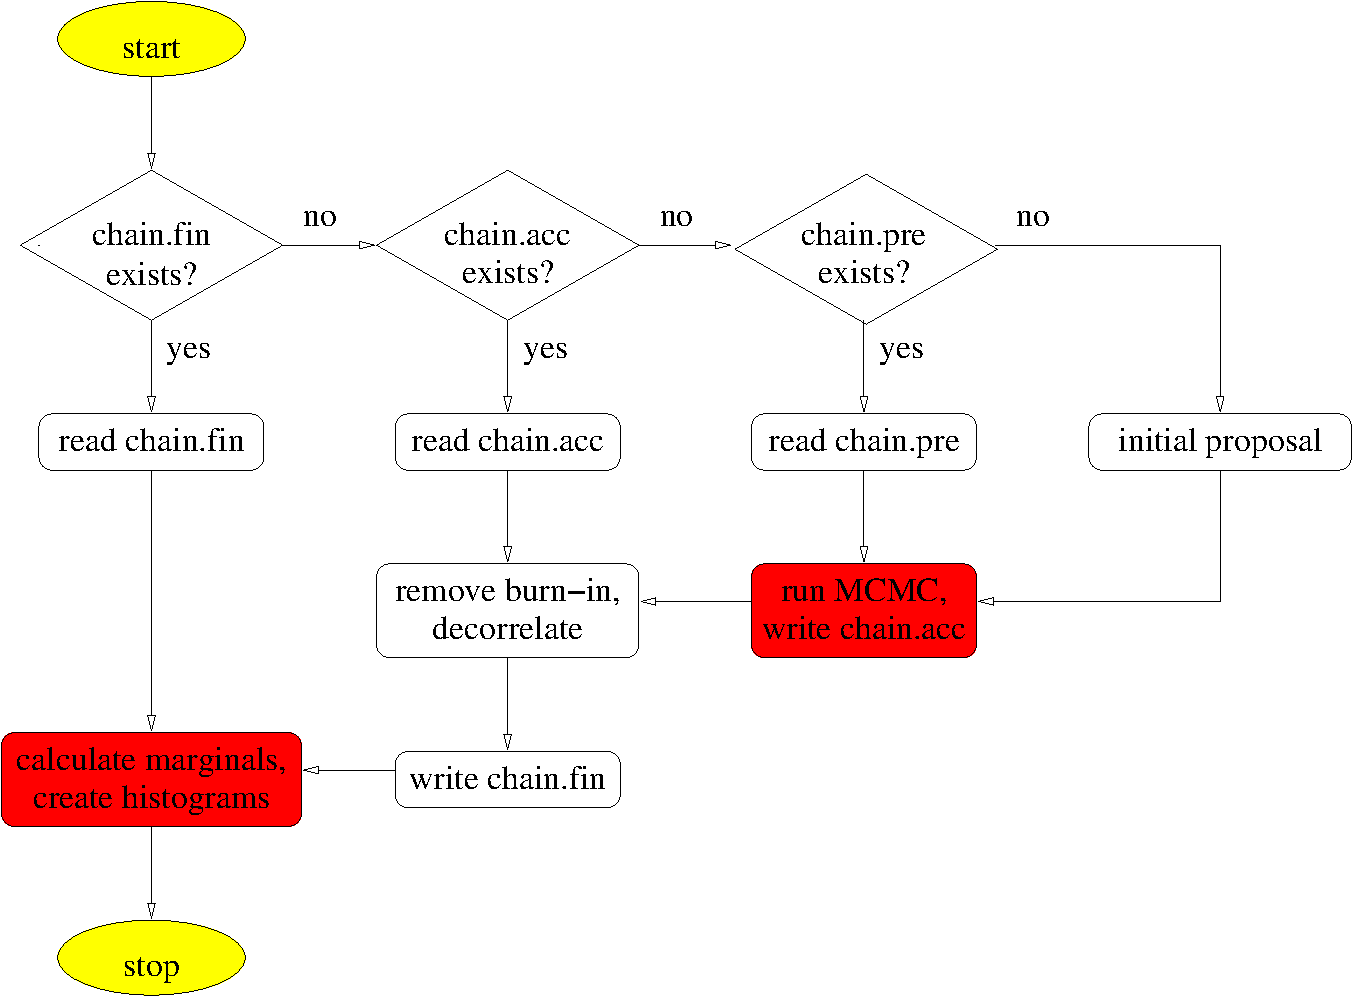
\includegraphics{chain_flow}
  }
  
  \caption{Flow chart of the MCMC implementation.}
  \label{fig:MCMC_flow}
\end{figure}


%%%%%%%%%%%%%%%%%%%%%%%%%%%%%%%%%%%%%%%%%%%%%%%%%%%%%%%%%%%%
\subsection{MCMC configuration file}
%%%%%%%%%%%%%%%%%%%%%%%%%%%%%%%%%%%%%%%%%%%%%%%%%%%%%%%%%%%%


\begin{table}
  \caption{MCMC section of the configuration file}
  \label{tab:MCMC}

\begin{minipage}{\textwidth}
  \begin{tabular}{llp{\spaltedrei}} \hline\hline
      %
    \texttt{nchain}  & integer & Chain Length\\
    \texttt{ncov}    & integer & Interval between updates of the proposal covariance \\
    \texttt{fburnin} & double & Burn-in phase are the first
                       \texttt{ncov}$\times$\texttt{ncor} points\\
    \texttt{ndecorr} & double & De-correlation (thinning-out): one in
    \texttt{ndec} points is kept in the final chain\\
    \texttt{fudge}   & double & Proposal covariance is multiplied by
    \texttt{fudge$^2$}/\texttt{n\_par} \\
    \texttt{sinitial} & string & Initial proposal type, one of
    \texttt{Fisher\_inv, Fisher, Fisher, previous, Hessian,
      Hessian\_diag, diag}. \\
    \texttt{boxdiv}\onlyif{sinitial}{diag} & double & Diagonal of proposal covariance is 
    \texttt{(max-min)/boxdiv} \\
    \texttt{sstart} & string & Starting point type, one of \texttt{ran,
      fid, min, max, nul} \\
    \texttt{fid}\onlyif{sstart}{fid} & \texttt{npar} doubles & Starting parameter \\
    \hline
    %
    \multicolumn{3}{c}{Histogram section} \\
    \hline
    %
    \texttt{nbinhist} & integer & Number of density histogram bins \\ \hline\hline
  \end{tabular}
\end{minipage}

\end{table}



%%%%%%%%%%%%%%%%%%%%%%%%%%%%%%%%%%%%%%%%%%%%%%%%%%%%%%%%%%%%
\subsection{Proposal and starting point}
\label{sec:mcmc_proposal}
%%%%%%%%%%%%%%%%%%%%%%%%%%%%%%%%%%%%%%%%%%%%%%%%%%%%%%%%%%%%

The proposal for the Metropolis-Hastings algorithm is a multi-variate
Gaussian distribution. After choosing an initial proposal, a new
proposal can optionally be re-calculated after a number of
\texttt{ncov} (accepted) steps. The covariance of this new proposal is
the chain covariance from steps up to this point. This proposal is
then updated after each \texttt{ncov} accepted steps using all
previous accepted points.

There are several options for the initial proposal:

\begin{enumerate}

\item \textbf{\texttt{sinitial = diag}} A diagonal
covariance with width being a fraction of the box size.

\item \textbf{\texttt{sinitial = Fisher}} The
Hessian at a given point in parameter space. If this point is the
maximum-likelihood point, the Hessian corresponds to the Fisher
matrix.

\item \textbf{\texttt{sinitial = Fisher\_inv}} The inverse
  Hessian/Fisher matrix, e.g.~the covariance from a previous
  chain. This can be useful for ill-conditioned matrices which are
  difficult to invert numerically.

\item \textbf{\texttt{sinitial = previous}} A proposal read from a
  file, e.g.\ from a previous MCMC run.

\end{enumerate}

%%%%%%%%%%%%%%%%%%%%%%%%%%%%%%%%%%%%%%%%%%%%%%%%%%%%%%%%%%%%
%\subsection{Metropolis-Hastings random walk}
%%%%%%%%%%%%%%%%%%%%%%%%%%%%%%%%%%%%%%%%%%%%%%%%%%%%%%%%%%%%

The starting point is either chosen randomly or specified in the
config file. The second case might be convenient if the prior volume
is very large and a very long burn-in phase is to be avoided. For
example, the ML-point or best-fit value from a previous experiment can
be chosen \cite{WMAP5-Dunkley08}.

%%%%%%%%%%%%%%%%%%%%%%%%%%%%%%%%%%%%%%%%%%%%%%%%%%%%%%%%%%%%
\subsection{Output files}
%%%%%%%%%%%%%%%%%%%%%%%%%%%%%%%%%%%%%%%%%%%%%%%%%%%%%%%%%%%%

The MCMC output files have the same format as their PMC counterparts (see Sect.~\ref{sec:pmc_samples}).

A complete run of \progr{cosmo\_mcmc} produces three files containing
the points of the Markov chain:

\begin{enumerate}
\item \file{chain.all} containing all, accepted and rejected, sample
  points. This is the only chain file will not be read or used in subsequent calls of
  \file{cosmo\_mcmc}.

  \item \file{chain.acc} containing the accepted points.

  \item \file{chain.fin} containing the accepted points after
    removal of the burn-in phase and after de-correlating
    (thinning-out) the chain. The results produced by \progr{cosmo\_mcmc}
    (mean, errors, histograms, covariance) are based on this file.
\end{enumerate}

The chains are \texttt{ASCII}-files, in the same format as the PMC
sample files. All weights are 1, and the second column contains the
log-likelihood (only in \file{chain.all}.


The parameter mean and confidence intervals are printed to the file
\file{mean}. The names of files containing the histograms and parameter
covariances are the same as for PMC.


%%%%%%%%%%%%%%%%%%%%%%%%%%%%%%%%%%%%%%%%%%%%%%%%%%%%%%%%%%%%
%\subsubsection{Other files}
%%%%%%%%%%%%%%%%%%%%%%%%%%%%%%%%%%%%%%%%%%%%%%%%%%%%%%%%%%%%

%\begin{itemize}

%  \item A log file \file{log\_mcmc}.

% \item \file{mcmc\_variance} contains the MCMC variance.

%\end{itemize}


%%%%%%%%%%%%%%%%%%%%%%%%%%%%%%%%%%%%%%%%%%%%%%%%%%%%%%%%%%%%
\subsection{Diagnostics}
%%%%%%%%%%%%%%%%%%%%%%%%%%%%%%%%%%%%%%%%%%%%%%%%%%%%%%%%%%%%

In general it is not straight-forward to diagnose an MCM chain. There
exists tests but no formal proofs for convergence
(e.g.~Gellman-Rubin), which in addition require very long or multiple
chains. We have not implemented such tests in the code. However,
there are a few (rather hand-waving) diagnostic tools to check the
reliability of an MCMC run.

Firstly, the acceptance rate $\eta$ should be in the range between
15\% and 25\%. A larger $\eta$ most probably corresponds to a chain
which stayed mainly in the high-density region and strongly
under-sampled the lower-density posterior regions. In that case the
error bars will be underestimated. A very small $\eta$ means probably
an under-sampling of the posterior since only few points are
accepted. However, this need not cause a bias for the parameters and
errors if the chain has been run long enough.


%%%%%%%%%%%%%%%%%%%%%%%%%%%%%%%%%%%%%%%%%%%%%%%%%%%%%%%%%%%%
\subsection{Resuming an interrupted run}
%%%%%%%%%%%%%%%%%%%%%%%%%%%%%%%%%%%%%%%%%%%%%%%%%%%%%%%%%%%%

Sometimes a MCMC run is interrupted before finishing, or one wishes a
previous run to be extended, for example because its convergence is
doubted. The MCMC program allows to read in and extend a previous
chain. To that end, rename the file \file{chain.acc} into
\file{chain.pre}. The proposal for the resumed run can but need not
be calculated from the previous chain (to be controlled in the config
file, see Sect.\ref{sec:mcmc_proposal}). In the config file, the
number of desired sample points has to be larger than the previous
chain.

\end{appendix}




%%%%%%%%%%%%%%%%%%%%%%%%%%%%%%%%%%%%%%%%%%%%%%%%%%%%%%%%%%%%
%%%%%%%%%%%%%%%%%%%%%%%%%%%%%%%%%%%%%%%%%%%%%%%%%%%%%%%%%%%%
\end{document}
%%%%%%%%%%%%%%%%%%%%%%%%%%%%%%%%%%%%%%%%%%%%%%%%%%%%%%%%%%%%
%%%%%%%%%%%%%%%%%%%%%%%%%%%%%%%%%%%%%%%%%%%%%%%%%%%%%%%%%%%%
